\documentclass[12pt,a4paper]{article}
\usepackage[T1]{fontenc}
\usepackage{amsmath,amssymb,mathrsfs,tikz,times,pifont}
\usepackage{enumitem}
\usepackage{multicol}
\usepackage{lmodern}
\usetikzlibrary{trees}
\newcommand\circitem[1]{%
\tikz[baseline=(char.base)]{
\node[circle,draw=gray, fill=red!55,
minimum size=1.2em,inner sep=0] (char) {#1};}}
\newcommand\boxitem[1]{%
\tikz[baseline=(char.base)]{
\node[fill=cyan,
minimum size=1.2em,inner sep=0] (char) {#1};}}
\setlist[enumerate,1]{label=\protect\circitem{\arabic*}}
\setlist[enumerate,2]{label=\protect\boxitem{\alph*}}
%%%::::::by chnini ameur :::::::%%%
\everymath{\displaystyle}
\usepackage[left=1cm,right=1cm,top=1cm,bottom=1.7cm]{geometry}
\usepackage[colorlinks=true, linkcolor=blue, urlcolor=blue, citecolor=blue]{hyperref}
\usepackage{array,multirow}
\usepackage[most]{tcolorbox}
\usepackage{varwidth}
\usepackage{float} %pour utiliser l'option [H] qui force l'image à apparaître exactement à l'endroit où elle est placée dans le code.
\tcbuselibrary{skins,hooks}
\usetikzlibrary{patterns}
%%%::::::by chnini ameur :::::::%%%
\newtcolorbox{exa}[2][]{enhanced,breakable,before skip=2mm,after skip=5mm,
colback=yellow!20!white,colframe=black!20!blue,boxrule=0.5mm,
attach boxed title to top left ={xshift=0.6cm,yshift*=1mm-\tcboxedtitleheight},
fonttitle=\bfseries,
title={#2},#1,
% varwidth boxed title*=-3cm,
boxed title style={frame code={
\path[fill=tcbcolback!30!black]
([yshift=-1mm,xshift=-1mm]frame.north west)
arc[start angle=0,end angle=180,radius=1mm]
([yshift=-1mm,xshift=1mm]frame.north east)
arc[start angle=180,end angle=0,radius=1mm];
\path[left color=tcbcolback!60!black,right color = tcbcolback!60!black,
middle color = tcbcolback!80!black]
([xshift=-2mm]frame.north west) -- ([xshift=2mm]frame.north east)
[rounded corners=1mm]-- ([xshift=1mm,yshift=-1mm]frame.north east)
-- (frame.south east) -- (frame.south west)
-- ([xshift=-1mm,yshift=-1mm]frame.north west)
[sharp corners]-- cycle;
},interior engine=empty,
},interior style={top color=yellow!5}}
%%%%%%%%%%%%%%%%%%%%%%%
\usepackage{fancyhdr}
\usepackage{eso-pic}         % Pour ajouter des éléments en arrière-plan
% Commande pour ajouter du texte en arrière-plan
\usepackage{tkz-tab}
\AddToShipoutPicture{
    \AtTextCenter{%
        \makebox[0pt]{\rotatebox{80}{\textcolor[gray]{0.7}{\fontsize{5cm}{5cm}\selectfont PGB}}}
    }
}
\usepackage{lastpage}
\fancyhf{}
\pagestyle{fancy}
\renewcommand{\footrulewidth}{1pt}
\renewcommand{\headrulewidth}{0pt}
\renewcommand{\footruleskip}{10pt}
\fancyfoot[R]{
\color{blue}\ding{45}\ \textbf{2025}
}
\fancyfoot[L]{
\color{blue}\ding{45}\ \textbf{Prof:M. BA}
}
\cfoot{\bf
\thepage /
\pageref{LastPage}}
% Création du compteur pour les exercices
\newcounter{probleme}
\renewcommand{\theprobleme}{\arabic{probleme}}  % Définit l'affichage du compteur en chiffres arabes

% Définir la commande \exo
\newcommand{\exo}{\refstepcounter{probleme}\textbf{Problème \theprobleme} }
\begin{document}
\renewcommand{\arraystretch}{1.5}
\renewcommand{\arrayrulewidth}{1.2pt}
\begin{tikzpicture}[overlay,remember picture]
    \node[draw=blue,line width=1.2pt,fill=purple,text=blue,inner sep=3mm,rounded corners,pattern=dots]at ([yshift=-2.5cm]current page.north) {\begingroup\setlength{\fboxsep}{0pt}\colorbox{white}{\begin{tabular}{|*1{>{\centering \arraybackslash}p{0.28\textwidth}} |*2{>{\centering \arraybackslash}p{0.2\textwidth}|} *1{>{\centering \arraybackslash}p{0.19\textwidth}|} }
                \hline
                \multicolumn{3}{|c|}{$\diamond$$\diamond$$\diamond$\ \textbf{Lycée de Dindéfélo}\ $\diamond$$\diamond$$\diamond$ } & \textbf{A.S. : 2025/2026}                                              \\ \hline
                \textbf{Matière: Mathématiques}                                                                                    & \textbf{Niveau : T}\textbf{S2} & \textbf{Date: 29/12/2025} & \textbf{} \\ \hline
                \multicolumn{4}{|c|}{\parbox[c]{10cm}{\begin{center}
                                                                  \textbf{{\Large\sffamily Td Limites ln}}
                                                              \end{center}}}                                                                                                        \\ \hline
            \end{tabular}}\endgroup};
\end{tikzpicture}

\vspace{3cm}
\fbox{\textbf{\exo}}

\underline{\textbf{Partie A}}
Soit $g$ la fonction numérique définie sur $]0; +\infty[$ par $g(x) = x(1 + \ln x)^2 - 1$.
\begin{enumerate}
    \item On admettra que $g$ est dérivable sur $]0; +\infty[$.
    \begin{enumerate}
        \item Calculer $g'(x)$ pour tout $x \in ]0; +\infty[$.
        \item Vérifier que pour tout $x \in ]0; +\infty[$, $g'(x) = (1 + \ln x)(3 + \ln x)$.
        \item Étudier le signe de $g'(x)$ suivant les valeurs de $x$ et en déduire le sens de variation de $g$.
    \end{enumerate}
    \item Dresser le tableau de variation de $g$. (On ne calculera pas les limites en $0$ et $+\infty$).
    \item 
    \begin{enumerate}
        \item Calculer $g(1)$.
        \item En déduire que pour tout $x \in ]0; 1[$, $g(x) < 0$ et pour tout $x \in ]1; +\infty[$, $g(x) > 0$.
    \end{enumerate}
\end{enumerate}

\underline{\textbf{Partie B}}
Soit $f$ la fonction définie par :
\[
\begin{cases} 
f(x) = x + \frac{1}{1 + \ln x} - 1 & \text{si } x \in ]0; \frac{1}{e}[ \cup ]\frac{1}{e}; +\infty[ \\
f(0) = -1
\end{cases}
\]
$(C)$ est la représentation graphique dans le repère orthonormé $(O, I, J)$ (unités : 2cm).
\begin{enumerate}
    \item 
    \begin{enumerate}
        \item Montrer que $f$ est continue en 0.
        \item Étudier la dérivabilité de $f$ en 0.
        \item En déduire la tangente à $(C)$ au point $A(0; -1)$.
    \end{enumerate}
    \item 
    \begin{enumerate}
        \item Calculer $\lim\limits_{x \to \frac{1}{e}^-} f(x)$, $\lim\limits_{x \to \frac{1}{e}^+} f(x)$ et $\lim\limits_{x \to +\infty} f(x)$.
        \item Montrer que la droite $(\Delta)$ d'équation $y = x - 1$ est une asymptote à $(C)$.
        \item Étudier les positions relatives de $(C)$ et $(\Delta)$.
        \item Préciser l'autre asymptote à la courbe $(C)$ de $f$.
    \end{enumerate}
    \item 
    \begin{enumerate}
        \item Montrer que pour tout $x \in ]0; +\infty[ \setminus \{\frac{1}{e}\}$, $f'(x) = \frac{g(x)}{x(1 + \ln x)^2}$.
        \item En déduire le sens de variation de $f$.
        \item Dresser son tableau de variation.
    \end{enumerate}
\end{enumerate}

\underline{\textbf{Partie C}}
\begin{enumerate}
    \item Calculer la dérivée de la fonction $h$ définie sur $]\frac{1}{e}; +\infty[$ par $h(x) = \ln(1 + \ln x)$.
    \item 
    \begin{enumerate}
        \item En déduire les primitives sur $]\frac{1}{e}; +\infty[$ de la fonction $k : x \mapsto \frac{f(x)}{x}$.
        \item Déterminer la primitive de $k$ qui prend la valeur $-1$ en 1.
    \end{enumerate}
\end{enumerate}

\fbox{\textbf{\exo}}

Le plan est muni d'un repère orthonormé $(O, I, J)$ d'unité graphique 2cm.

\underline{\textbf{Partie A : Étude d'une fonction auxiliaire}}

Soit $g$ la fonction définie sur l'intervalle $]0; +\infty[$ par $g(x) = x^2 - 1 + \ln x$.
\begin{enumerate}
    \item Calculer $g'(x)$ pour tout réel $x$ appartenant à l'intervalle $]0; +\infty[$. \\
    En déduire le sens de variation de la fonction $g$ sur l'intervalle $]0; +\infty[$.
    \item Calculer $g(1)$ et en déduire l'étude du signe de $g(x)$ pour $x$ appartenant à $]0; +\infty[$.
\end{enumerate}

\underline{\textbf{Partie B : Détermination de l'expression de la fonction $f$}}

On admet qu'il existe deux constantes réelles $a$ et $b$ telles que, pour tout nombre réel $x$ appartenant à $]0; +\infty[$, $f(x) = ax + b - \frac{\ln x}{x}$.
\begin{enumerate}
    \item On désigne par $f'$ la fonction dérivée de la fonction $f$. \\
    Calculer $f'(x)$ pour tout réel $x$ appartenant à l'intervalle $]0; +\infty[$.
    \item Sachant que la courbe $(C)$ passe par le point de coordonnées $(1; 0)$ et qu'elle admet en ce point une tangente horizontale, déterminer les nombres $a$ et $b$.
\end{enumerate}

\underline{\textbf{Partie C : Étude de la fonction $f$}}

On admet désormais que, pour tout nombre réel $x$ appartenant à l'intervalle $]0; +\infty[$, $f(x) = x - 1 - \frac{\ln x}{x}$.
\begin{enumerate}
    \item 
    \begin{enumerate}
        \item Déterminer la limite de la fonction $f$ en $0$ et donner une interprétation graphique de cette limite.
        \item Déterminer la limite de la fonction $f$ en $+\infty$.
    \end{enumerate}
    \item 
    \begin{enumerate}
        \item Vérifier que, pour tout réel $x$ appartenant à l'intervalle $]0; +\infty[$, $f'(x) = \frac{g(x)}{x^2}$.
        \item Établir le tableau de variation de la fonction $f$ sur l'intervalle $]0; +\infty[$.
        \item En déduire le signe de $f(x)$ pour $x$ appartenant à l'intervalle $]0; +\infty[$.
    \end{enumerate}
    \item On considère la droite $(D)$ d'équation $y = x - 1$.
    \begin{enumerate}
        \item Justifier que la droite $(D)$ est asymptote à la courbe $(C)$.
        \item Étudier les positions relatives de la courbe $(C)$ et de la droite $(D)$.
        \item Tracer la droite $(D)$ et la courbe $(C)$ dans le plan $P$ muni du repère $(O; \vec{i}, \vec{j})$.
    \end{enumerate}
\end{enumerate}

\underline{\textbf{Partie D : Calcul d'aire}}

On note $A$ la mesure, exprimée en $cm^2$, de l'aire de la partie du plan $P$ comprise entre la courbe $C$, l'axe des abscisses, et les droites d'équations $x = 1$ et $x = e$.
\begin{enumerate}
    \item On considère la fonction $H$ définie sur l'intervalle $]0; +\infty[$ par $H(x) = (\ln x)^2$. \\
    On désigne par $H'$ la fonction dérivée de la fonction $H$.
    \begin{enumerate}
        \item Calculer $H'(x)$ pour tout réel $x$ appartenant à l'intervalle $]0; +\infty[$.
        \item En déduire une primitive de la fonction $f$ sur l'intervalle $]0; +\infty[$.
    \end{enumerate}
    \item Calculer $A$ et donner sa valeur arrondie au $mm^2$ près.
\end{enumerate}

\fbox{\textbf{\exo}}

\underline{\textbf{Partie A}}
On considère $g$ la fonction numérique de la variable réelle $x$ définie par :
\[ g(x) = 1 + x(2\ln|x| + 1) \]

\begin{enumerate}
    \item 
    \begin{enumerate}
        \item Justifier que $g$ est définie sur $]-\infty; 0[ \cup ]0; +\infty[$.
        \item Déterminer les limites de $g$ aux bornes de son ensemble de définition.
    \end{enumerate}
    \item 
    \begin{enumerate}
        \item Étudier le sens de variation de $g$.
        \item Dresser le tableau de variation de $g$.
    \end{enumerate}
    \item 
    \begin{enumerate}
        \item Calculer l'image de $-1$ par $g$.
        \item Déterminer l'image $J$ par $g$ de l'intervalle $I$ tel que : $I = ]-\infty; -e^{-\frac{3}{2}}]$.
        \item Démontrer que la restriction $h$ de $g$ sur l'intervalle $I$ est une bijection de $I$ sur $J$.
        \item En déduire l'ensemble des solutions de l'équation : $x \in \mathbb{R}, g(x) = 0$.
    \end{enumerate}
    \item Déduire de tout ce qui précède que : \\
    $\forall x \in ]-\infty; -1[, g(x) < 0$ et $\forall x \in ]-1; 0[ \cup ]0; +\infty[, g(x) > 0$.
\end{enumerate}

\underline{\textbf{Partie B}}
On considère $f$ la fonction numérique de la fonction de la variable réelle $x$ définie par :
\[
\begin{cases}
f(x) = x(x\ln|x| + 1) & \text{si } x \neq 0 \\
f(0) = 0
\end{cases}
\]
et $(C)$ sa courbe représentative dans le plan muni du repère orthonormé $(O; \vec{i}, \vec{j})$. (Unité : 5cm)

\begin{enumerate}
    \item Démontrer que $f$ est continue en 0.
    \item 
    \begin{enumerate}
        \item Donner l'ensemble de définition de $f'$ et déterminer les limites de $f$ aux bornes de son ensemble de définition.
        \item Étudier la dérivabilité de $f$ en 0.
        \item Déterminer la fonction dérivée $f'$ et déterminer le tableau de variation de $f$.
    \end{enumerate}
    \item 
    \begin{enumerate}
        \item Écrire une équation de la tangente $(D)$ à la courbe $(C)$ au point $O$.
        \item Démontrer que $(D)$ coupe $(C)$ en deux points $E$ et $F$ et calculer leurs coordonnées.
        \item Étudier la position de $(C)$ par rapport à $(D)$.
    \end{enumerate}
    \item Démontrer que $(C)$ coupe l'axe $(OI)$ en un point $K$ d'abscisse $\beta$ tel que $-1,8 < \beta < -1,7$.
    \item Construire $(C)$.
\end{enumerate}

\underline{\textbf{Partie C}}
\begin{enumerate}
    \item Soit $\alpha$ un réel appartenant à $]0; 1[$. \\
    À l'aide d'une intégration par parties, calculer $\int_{\alpha}^{1} x^2 \ln(x) \, dx$.
    \item 
    \begin{enumerate}
        \item Calculer l'aire $A(\alpha)$ de la partie du plan limitée par $(C)$, la droite $(D)$ et les droites d'équation $x = 1$ et $x = \alpha$.
        \item Calculer $\lim\limits_{\alpha \to 0} A(\alpha)$.
    \end{enumerate}
\end{enumerate}

\begin{center}
    On prendra : $\ln(2) \approx 0,7$ ; $\ln(3) \approx 1,1$ ; $\ln(5) \approx 1,6$ ; $\ln(17) \approx 2,9$ ; $e \approx 2,7$ ; $\sqrt{e} \approx 1,6$.
\end{center}
\fbox{\textbf{\exo}}

\noindent \underline{\textbf{Partie A}} \\
On considère la fonction $g$ dérivable et définie sur $\mathbb{R}^*$ par :
\[ g(x) = -x^3 + x + 1 - \ln|x| \]
\begin{enumerate}
    \item Montrer que $-1$ est un zéro de la fonction polynôme $P$ définie par : $P(x) = -3x^3 + x - 2$.
    \item \begin{enumerate}
        \item Déterminer le signe de $P(x)$ suivant les valeurs de $x$.
        \item Calculer les limites de $g$ aux bornes des intervalles de son ensemble de définition.
        \item Étudier les variations de $g$.
        \item Montrer que l'équation $g(x) = 0$ admet une solution unique. On note $\alpha$ cette solution. \\
        Montrer que : $1,2 < \alpha < 1,3$.
        \item En déduire que : $\forall x \in ]-\infty; 0[ \cup ]0; \alpha[, g(x) > 0$ ; $\forall x \in ]\alpha; +\infty[, g(x) < 0$.
    \end{enumerate}
\end{enumerate}

\vspace{0.5cm}
\noindent \underline{\textbf{Partie B}} \\
On considère la fonction $f$ dérivable et définie sur $\mathbb{R}^*$ par :
\[ f(x) = -x + 1 - \frac{x - \ln|x|}{x^2} \]
On appelle $(C)$ la courbe représentative de $f$ dans un repère orthonormé $(O, I, J)$. (Unité graphique : 2cm)
\begin{enumerate}
    \item Calculer les limites de $f$ aux bornes des intervalles de son ensemble de définition.
    \item \begin{enumerate}
        \item Démontrer que pour tout $x \in \mathbb{R}^*$, $f'(x) = \frac{g(x)}{x^3}$.
        \item Étudier les variations de $f$ et dresser son tableau de variation.
    \end{enumerate}
    \item Déterminer une équation de la tangente $(T)$ au point d'abscisse $-1$.
    \item Déterminer que la droite $(D)$ d'équation $y = -x + 1$ est asymptote à la courbe $(C)$.
    \item \begin{enumerate}
        \item Étudier les variations de la fonction $h$ définie sur $\mathbb{R}^*$ par : $h(x) = x - \ln|x|$.
        \item En déduire que $(D)$ coupe $(C)$ en un point unique d'abscisse $\beta$ vérifiant : $\ln(-\beta) = \beta$.
        \item Montrer que : $-0,57 < \beta < 0,56$.
        \item Déterminer la position de $(C)$ par rapport à $(D)$.
    \end{enumerate}
    \item Construire $(T)$, $(D)$ et $(C)$.
    \item Démontrer que la fonction numérique $F$ définie sur $]0; +\infty[$ par : \\
    $F(x) = -\frac{1}{2}x^2 + x - \frac{1}{x} - \ln x - \frac{(\ln x)^2}{x}$ est une primitive de $f$ sur $]0; +\infty[$.
\end{enumerate}

\begin{center}
    \fbox{\textbf{\exo}}
\end{center}

\vspace{0.5cm}

\noindent \underline{\textbf{Partie A}} \\
Soit $g$, la fonction de $\mathbb{R}$ vers $\mathbb{R}$ définie par $g(x) = (x+2)^2 + \ln|x+2|$.
\begin{enumerate}
    \item \begin{enumerate}
        \item Calculer les limites de $g$ au borne de son ensemble de définition.
        \item Etudier les variations de $g$ sur $]-2; +\infty[$.
    \end{enumerate}
    \item \begin{enumerate}
        \item Montrer que l'équation $g(x) = 0$ admet une solution unique $\beta$ dans $]-2; +\infty[$.
        \item Montrer que $\beta$ vérifie $-1,35 < \beta < -1,34$.
        \item Déterminer le signe de $g(x)$ sur $]-2; +\infty[$.
    \end{enumerate}
\end{enumerate}

\vspace{0.5cm}

\noindent \underline{\textbf{Partie B}} \\
Soit $f$ la fonction définie par $f(x) = -x - 1 + \frac{1 + \ln(x+2)}{x+2}$ et $(\varepsilon)$ sa courbe représentative dans le plan muni du repère orthonormé $(O, I, J)$. Unité 2 centimètres.
\begin{enumerate}
    \item \begin{enumerate}
        \item Déterminer l'ensemble de définition de $f$ et la limite de $f$ en $+\infty$.
        \item Déterminer la limite de $f$ à droite en $-2$. Interpréter graphiquement le résultat.
        \item Montrer que, $\forall x \in ]-2; +\infty[ ; f'(x) = \frac{-g(x)}{(x+2)^2}$. En déduire le signe de $f'(x)$ et dresser le tableau de variation de $f$.
        \item Montrer que $f(\beta) = -2\beta - 3 + \frac{1}{\beta+2}$.
    \end{enumerate}
    \item \begin{enumerate}
        \item Montre que la droite $(D) : y = -x - 1$ est asymptote à $(\varepsilon)$.
        \item Déterminer les coordonnées de $A$ intersection de $(\varepsilon)$ et de $(D)$.
        \item Etudier la position de $(\varepsilon)$ par rapport à $(D)$.
    \end{enumerate}
    \item Construire $(\varepsilon)$ et $(D)$ sur le même graphique.
    \item Déterminer $G$, la primitive de $g(x)$ tel que $g(x) = (x+2)^2 + \ln(x+2)$ sur $]-2; +\infty[$ et s'annule en $-1$. \\
    Sachant que la primitive sur $]-2; +\infty[$ de $\ln(x+2)$ est $(x+2)\ln(x+2) - (x+2)$.
    \item \begin{enumerate}
        \item Si $h$ est la restriction de $f$ à l'intervalle $[\beta; +\infty[$, montrer que $h$ est une bijection de $[\beta; +\infty[$ sur une partie $K$ que l'on déterminera.
        \item Calculer $h(-1)$.
        \item Montrer $h^{-1}$ est dérivable en 1 et calculer $(h^{-1})'(1)$.
        \item Construire $(\varepsilon')$, la représentation graphique de $h^{-1}$, bijection réciproque de $h$ sur le graphique précédent.
    \end{enumerate}
\end{enumerate}

\begin{center}
    \fbox{\textbf{\exo}}
\end{center}

\vspace{0.5cm}

\noindent \underline{\textbf{Partie A :}} Etude d'une fonction numérique de la variable réelle $x$ définie par :
\[ f(x) = \left(x - \frac{1}{2}\right)e^{2x} - 4(x - 1)e^x - 2 \]

\begin{enumerate}
    \item \begin{enumerate}
        \item Calculer la limite de $f$ en $-\infty$.
        \item Montrer que $f(x) = xe^{2x} \left( 1 - \frac{1}{2x} - \frac{4}{e^x} + \frac{4}{xe^x} - \frac{2}{xe^{2x}} \right)$ et en déduire la limite de $f$ en $+\infty$.
    \end{enumerate}
    \item Etudier les variations de $f$.
    \item Soit $(C_f)$ la courbe représentative de $f$ dans le repère orthonormé, unité graphique 2cm.
    \begin{enumerate}
        \item Etudier les branches infinies de $(C_f)$.
        \item Montrer que $(C)$ coupe l'axe des abscisses en un point, dont l'abscisse $\alpha$ appartient à l'intervalle $[-2; -1]$.
        \item Tracer $(C_f)$. On prendra $\ln 2 \approx 0,7$.
    \end{enumerate}
    \item Montrer que $F(x) = \left(\frac{x}{2} - \frac{1}{2}\right)e^{2x} + 4(2 - x)e^x$ est une primitive de $f(x) + 2$.
\end{enumerate}

\vspace{0.8cm}

\noindent \underline{\textbf{Partie B :}} Etude d'une nouvelle fonction numérique de variable réelle $x$ définie par :
\[
\begin{cases} 
g(x) = (x^2 - 4x)\ln x - \dfrac{1}{2}(x^2 - 8x + 4) & \forall x > 0 \\
g(0) = -2 
\end{cases}
\]

\begin{enumerate}
    \item Montrer que : $g(x) = f(\ln x), \forall x > 0$.
    \item Etudier la continuité et la dérivabilité de $g$ à droite en 0.
    \item Calculer les limites aux bornes de son domaine.
    \item Etudier les variations de $g$.
    \item Soit $(C_g)$ la courbe représentative de $g$ dans un repère orthonormé, unité 2cm.
    \begin{enumerate}
        \item Etudier la branche infinie de $(C_g)$.
    \end{enumerate}
\end{enumerate}

\begin{center}
    \fbox{\textbf{\exo}}
\end{center}

\noindent Soit $f$ la fonction numérique à variable réelle définie par : $f(x) = \dfrac{1}{1-xe^{-x}}$ \\
On note $(C)$ sa courbe représentative dans un repère orthonormé direct $(O, I, J)$. Unité graphique : 2cm

\vspace{0.5cm}

\noindent \underline{\textbf{Partie A}} \\
Soit $g$ la fonction définie sur $\mathbb{R}$ par : $g(x) = 1 - xe^{-x}$
\begin{enumerate}
    \item Démontrer que : $\forall x \in \mathbb{R}, g'(x) = (x - 1)e^{-x}$
    \item Déterminer le sens de variation de $g$ puis, dresser le tableau de variation de $g$ (sans les limites aux bornes).
    \item Démontrer que : $\forall x \in \mathbb{R}, g(x) > 0$.
\end{enumerate}

\vspace{0.8cm}

\noindent \underline{\textbf{Partie B}}
\begin{enumerate}
    \item Démontrer que l'ensemble de définition de $f$ est $\mathbb{R}$.
    \item Calculer la limite de $f$ en $-\infty$ et en $+\infty$. En donner une interprétation graphique.
    \item \begin{enumerate}
        \item Démontrer que : $\forall x \in \mathbb{R}, f'(x) = \dfrac{(1-x)e^{-x}}{(1-xe^{-x})^2}$.
        \item Déterminer le sens de variation de $f$ puis dresser le tableau de variation de $f$.
    \end{enumerate}
    \item \begin{enumerate}
        \item Démontrer qu'une équation de la tangente $(T)$ au point d'abscisse 0 est $y = x + 1$.
        \item Démontrer que : $\forall x \in \mathbb{R}, f(x) - x - 1 = \dfrac{(x+1-e^x)xe^{-x}}{1-xe^{-x}}$.
        \item Déterminer le signe de la fonction $h$ telle que : $h(x) = x + 1 - e^{-x}$.
        \item Déduire de la question précédente les positions relatives de $(C)$ et de $(T)$.
    \end{enumerate}
    \item Construire $(T)$ et $(C)$.
\end{enumerate}
\begin{center}
    \fbox{\textbf{\exo}}
\end{center}

\noindent \underline{\textbf{Partie A :}} (Etude d'une fonction auxiliaire $g$) \\
Soit $g$ la fonction numérique définie sur $]0; +\infty[$ par : 
\( g(x) = x - 2 - 2x\ln x \)
\begin{enumerate}
    \item Justifier que l'ensemble des solutions de l'inéquation : 
    $-2\ln x - 1 \ge 0$ est $S = \left] 0; e^{-\frac{1}{2}} \right]$
    \item \begin{enumerate}
        \item Calculer $g'(x)$.
        \item Etudier les variations de $g$.
    \end{enumerate}
    \item \begin{enumerate}
        \item Etablir le tableau de variation de $g$. (On ne cherchera pas à calculer les limites de $g$).
        \item En déduire que : $\forall x \in ]0; +\infty[, g(x) < 0$.
    \end{enumerate}
\end{enumerate}

\vspace{0.8cm}

\noindent \underline{\textbf{Partie B :}} (Etude et représentation graphique d'une fonction $f$) \\
Soit $f$ la fonction numérique définie sur $[0; +\infty[$ par : 
$f(x) = (x - 1)^2 - x^2\ln x$ si $x \in ]0; +\infty[$ et $f(0) = 1$. \\
On note $(C)$ la courbe représentative de $f$ dans le plan muni du repère orthonormé $(O, I, J)$. \\
L'unité graphique est 2cm.
\begin{enumerate}
    \item \begin{enumerate}
        \item Calculer la limite de $f$ en $+\infty$.
        \item Justifier que la courbe $(C)$ admet en $+\infty$ une branche parabolique dont on précisera la direction.
    \end{enumerate}
    \item \begin{enumerate}
        \item Justifier que $f$ est continue en 0.
        \item Démontrer que $\lim\limits_{x \to 0} \dfrac{f(x) - f(0)}{x - 0} = -2$.
    \end{enumerate}
    \item Soit $(T)$ la droite d'équation $y = -2x + 1$ et $d$ la fonction définie sur $]0; +\infty[$ par $d(x) = f(x) - y$.
    \begin{enumerate}
        \item Justifier que $(T)$ est la tangente à la courbe $(C)$ au point d'abscisse 0.
        \item Vérifier que pour tout $x \in ]0; +\infty[, d(x) = x^2 - x^2\ln x$.
        \item Etudier la position relative de $(C)$ par rapport à $(T)$.
    \end{enumerate}
    \item \begin{enumerate}
        \item Démontrer que : $\forall x \in ]0; +\infty[, f'(x) = g(x)$.
        \item Etablir le tableau de variation de la fonction $f$.
    \end{enumerate}
    \item \begin{enumerate}
        \item Démontrer que l'équation $f(x) = 0$ admet une unique solution $\alpha$ dans $]0; +\infty[$.
        \item Vérifier que $\alpha = 1$ et démontrer que $f(x) \ge 0$ si $0 \le x \le 1$ et $f(x) \le 0$ si $x \ge 1$.
    \end{enumerate}
    \item Construire $(T)$ et $(C)$.
\end{enumerate}

\vspace{0.8cm}

\noindent \underline{\textbf{Partie C :}} (Etude d'une primitive $F$ d'une restriction de la fonction $f$) \\
Soit $F$ la primitive de $f$ sur $[1; +\infty[$ qui s'annule en $e$. (On ne cherchera pas à déterminer $F$).
\begin{enumerate}
    \item Déterminer $F(e)$ et $F'(x)$. (On justifiera chaque réponse).
    \item Démontrer que $F$ est une bijection de $]1; +\infty[$ vers $F(]1; +\infty[)$.
    \item Soit $F^{-1}$ la réciproque de $F$. Calculer $(F^{-1})'(0)$.
\end{enumerate}


\begin{center}
    \fbox{\textbf{\exo}}
\end{center}

\noindent On désigne par $(C)$ la courbe de la fonction $f$ ci-dessous dérivable sur $\mathbb{R} \setminus \{0; 1\}$ dans le plan d'un repère orthonormé $(O; I, J)$. L'unité de longueur : 2 cm.

\vspace{0.2cm}

\noindent \underline{\textbf{Partie A :}} On considère la fonction $f$ définie par :
\( f(x) = x - 1 - \frac{2}{x} - \ln \left| 1 - \frac{1}{x} \right| \)

\begin{enumerate}
    \item Montrer que $f$ est définie sur $\mathbb{R} \setminus \{0; 1\}$.
    \item Montrer que :
    \begin{itemize}
        \item Pour tout $x \in ]-\infty; 0[ \cup ]1; +\infty[ ; f(x) = x - 1 - \frac{2}{x} - \ln\left( 1 - \frac{1}{x}\right) $
        \item Pour tout $x \in ]0; 1[ ; f(x) = x - 1 - \frac{2}{x} - \ln\left( \frac{1}{x} - 1\right) $
    \end{itemize}
    \item Déterminer les limites de $f$ en $-\infty$ et en $+\infty$.
    \item Calculer la limite de $f$ en 1. Interpréter graphiquement ce résultat.
    \item \begin{enumerate}
        \item Calculer les limites de $f$ à gauche en 0 et à droite en 0.
        \item Interpréter graphiquement ces résultats.
    \end{enumerate}
\end{enumerate}


\noindent \underline{\textbf{Partie B :}} Soit la fonction $g$ définie sur $\mathbb{R}$ par : $g(x) = x^3 - x^2 + x - 2$.
\begin{enumerate}
    \item Calculer $g'(x)$, $g'$ étant la fonction dérivée de $g$.
    \item Déterminer le sens de variation de $g$.
    \item \begin{enumerate}
        \item Montrer que l'équation $g(x) = 0$ admet une solution unique $\alpha$ dans $\mathbb{R}$ et que $1 < \alpha < 1,5$.
        \item En déduire un encadrement de $\alpha$ par deux décimaux consécutifs d'ordre 1.
    \end{enumerate}
    \item Montrer que pour tout $x \in ]-\infty; \alpha[ ; g(x) < 0$ et pour tout $x \in ]\alpha; +\infty[ ; g(x) > 0$.
    \item Montrer que pour tout nombre réel $x$ élément de $\mathbb{R} \setminus \{0; 1\}$, $f'(x) = \dfrac{g(x)}{x^2(x-1)}$.
    \item \begin{enumerate}
        \item Déterminer le signe de $f'(x)$.
        \item Dresser le tableau de variation de $f$.
    \end{enumerate}
\end{enumerate}


\noindent \underline{\textbf{Partie C}}
\begin{enumerate}
    \item Soit $(D)$ la droite d'équation $y = x - 1$. \\
    Montrer que la droite $(D)$ est une asymptote à $(C)$ en $-\infty$ et en $+\infty$.
    \item Calculer $f(-2) ; f(-\frac{1}{2})$ et $f(\frac{1}{2})$.
    \item Construire dans le repère $(O; I, J)$ la courbe $(C)$ et ses asymptotes. On prendra $\alpha \approx 1,3$.
\end{enumerate}

\noindent \underline{\textbf{Partie D}}\\
On considère les fonctions $h$ et $k$ définies sur $]2; +\infty[$ par $h(x) = (x - 1) \ln(x - 1) - x \ln x$ et on admettra que pour tout $x$ élément de $]2; +\infty[$, $f(x) - x + 1 < 0$.
\begin{enumerate}
    \item Calculer $h'(x)$, $h'$ étant la dérivée de $h$.
    \item Calculer l'aire de la partie limitée par la courbe $(C)$, la droite $(D)$ et les droites d'équations $x = 2$ et $x = 4$.
\end{enumerate}

\begin{center}
    \fbox{\textbf{\exo}}
\end{center}

\noindent Le plan est muni d'un repère orthonormé $(O, I, J)$. Unité : $OI = 2\text{cm}$ et $OJ = 1\text{cm}$.

\vspace{0.5cm}

\noindent \underline{\textbf{Partie A}} \\
Soit $g$ la fonction de $\mathbb{R}$ vers $\mathbb{R}$ définie par : $g(0) = -1$ et $g(x) = \dfrac{x}{(\ln(x))^2} - 1$ et $(C_g)$ sa courbe.

\begin{enumerate}
    \item \begin{enumerate}
        \item Déterminer l'ensemble de définition de $g$.
        \item Calculer les limites de $g$ en 1 et en $+\infty$.
        \item Calculer $\lim\limits_{x \to +\infty} \dfrac{g(x)}{x}$ puis interpréter graphiquement ce résultat.
    \end{enumerate}
    \item \begin{enumerate}
        \item Démontrer que $g$ est continue en 0.
        \item Étudier la dérivabilité de $g$ en 0 et interpréter graphiquement ce résultat.
    \end{enumerate}
    \item On admet que $g$ est dérivable sur $[0; 1[ \cup ]1; +\infty[$.
    \begin{enumerate}
        \item Démontrer que $\forall x \in ]0; 1[ \cup ]1; +\infty[ ; g'(x) = \dfrac{\ln(x)(\ln(x) - 2)}{(\ln(x))^4}$.
        \item Déterminer le sens de variation de $g$ puis dresser son tableau de variation.
    \end{enumerate}
    \item \begin{enumerate}
        \item Démontrer que l'équation $\forall x \in \mathbb{R}, g(x) = 0$ admet une unique solution $\alpha$ dans $]0; 1[$.
        \item Vérifier que $0,4 < \alpha < 0,5$.
        \item En déduire que : $\forall x \in [0; \alpha[ ; g(x) < 0$ \\
        $\forall x \in ]\alpha; 1[ \cup ]1; +\infty[ ; g(x) > 0$.
    \end{enumerate}
\end{enumerate}

\vspace{0.5cm}

\noindent \underline{\textbf{Partie B}} \\
On considère la fonction numérique $f$ définie sur $]0; 1[ \cup ]1; +\infty[$ par : $f(x) = \dfrac{1}{x} - \dfrac{1}{\ln(x)}$ et $(C)$, sa courbe.

\begin{enumerate}
    \item \begin{enumerate}
        \item Calculer les limites de $f$ en 0, en 1 et en $+\infty$.
        \item Interpréter graphiquement les résultats précédents.
    \end{enumerate}
    \item On admet que $f$ est dérivable sur $]0; 1[ \cup ]1; +\infty[$.
    \begin{enumerate}
        \item Démontrer que $\forall x \in ]0; 1[ \cup ]1; +\infty[ , f'(x) = \dfrac{g(x)}{x^2}$.
        \item Étudier le sens de variation de $f$ et dresser son tableau de variation de $f$.
    \end{enumerate}
    \item Démontrer que $f(\alpha) = \dfrac{1 - \sqrt{\alpha}}{\alpha}$. En déduire le signe de $f(x)$ sur $]0; 1[ \cup ]1; +\infty[$.
     \item Construire la courbe $(C)$. On prendra $\alpha \simeq 0,5$.
\end{enumerate}

\vspace{0.5cm}

\noindent \underline{\textbf{Partie C}} \\
Soit $h$ la restriction de $f$ à $]1; +\infty[$.

\begin{enumerate}
    \item Démontrer que $h$ est la bijection de $]1; +\infty[$ sur un intervalle $K$ que l'on déterminera.
    \item On note $h^{-1}$ la bijection réciproque de $h$ et $(\Gamma)$ sa représentation graphique.
    \begin{enumerate}
        \item Dresser le tableau de variation de $h^{-1}$.
        \item Calculer $h(e)$ ; $h^{-1}\left( \dfrac{1-e}{e}\right) $ et $(h^{-1})'\left( \dfrac{1-e}{e}\right) $.
        \item Déterminer une équation de la tangente $(T)$ à $(\Gamma)$ au point d'abscisse $\dfrac{1-e}{e}$.
    \end{enumerate}
    \item Construire $(\Gamma)$ dans le même repère que $(C)$.
\end{enumerate}

\begin{center}
    \fbox{\textbf{\exo}}
\end{center}

\vspace{0.5cm}

\noindent \underline{\textbf{Partie A}} \\
Soit $g$ la fonction définie sur $[0; +\infty[$ par : 
$\begin{cases} \forall x > 0, g(x) = 1 - x\ln x \\ g(0) = 1 \end{cases}$

\begin{enumerate}
    \item \begin{enumerate}
        \item Etudier la continuité de $g$ en 0.
        \item Etudier la dérivabilité de $g$ en 0. Interpréter graphiquement le résultat.
    \end{enumerate}
    \item Calculer la limite de $g$ en $+\infty$.
    \item Etudier les variations de $g$ et dresser son tableau de variations.
    \item \begin{enumerate}
        \item Montrer que l'équation $g(x)=0$ admet une unique solution $\alpha \in ]e^{-1}; +\infty[$.
        \item Justifier que : $1,7 < \alpha < 1,8$.
    \end{enumerate}
    \item Démontrer que : 
    $\begin{cases} \forall x \in [0; \alpha[, g(x) > 0 \\ \forall x \in [\alpha; +\infty[, g(x) < 0 \end{cases}$
\end{enumerate}

\vspace{0.8cm}

\noindent \underline{\textbf{Partie B}} \\
Soit $f$ la fonction définie sur $]0; +\infty[$ par : $f(x) = e^{3-x}\ln x$ \\
$(C_f)$ désigne sa représentation graphique dans le plan est muni d'un repère orthonormé $(O; I; J)$ Unité graphique : 2cm

\begin{enumerate}
    \item Calculer la limite de $f$ en 0. Interpréter graphiquement le résultat.
    \item \begin{enumerate}
        \item Vérifier que : $\forall x \in ]0; +\infty[ : f(x) = \left(\dfrac{\ln x}{x}\right) \left(\dfrac{x}{e^x}\right) e^3$
        \item En déduire la limite de $f$ en $+\infty$. Interpréter graphiquement le résultat.
    \end{enumerate}
    \item \begin{enumerate}
        \item Montrer que : $\forall x \in ]0; +\infty[, f'(x) = \dfrac{e^{3-x}}{x} g(x)$.
        \item En déduire le sens de variations de $f$.
    \end{enumerate}
    \item \begin{enumerate}
        \item Montrer que : $f(\alpha) = \dfrac{e^3}{\alpha e^{\alpha}}$.
        \item En déduire un encadrement de $f(\alpha)$.
        \item Dresser le tableau de variations de $f$.
    \end{enumerate}
     \item Construire $(C_f)$.
     \item Soit $h$ la restriction de $f$ à l'intervalle $]0; \alpha[$.
     \begin{enumerate}
            \item Montrer que $h$ admet une bijection réciproque $h^{-1}$ dont on précisera l'ensemble de départ, l'arrivée d'arrivée.
            \item Dresser le tableau de variation de $h^{-1}$.
            \item Calculer $(h^{-1})'(0)$.
      \end{enumerate}
\end{enumerate}

\begin{center}
    \fbox{\textbf{\exo}}
\end{center}

\vspace{0.3cm}

\noindent \underline{\textbf{Partie A}} \\
On considère l'équation différentielle (1) : $y' - 2y = xe^x$
\begin{enumerate}
    \item Résoudre l'équation différentielle (2) : $y' - 2y = 0$
    \item Soient $a$ et $b$ deux réels et soit $u$ la fonction définie sur $\mathbb{R}$ par $u(x) = (ax + b)e^x$.
    \begin{enumerate}
        \item Déterminer $a$ et $b$ pour que $u$ soit solution de l'équation (1).
        \item Montrer que $v$ est une solution de l'équation (1) si et seulement si $u+v$ est une solution de l'équation (2).
        \item En déduire l'ensemble des solutions de l'équation (1).
    \end{enumerate}
    \item Déterminer la solution $f$ de l'équation (1) qui s'annule en 0.
\end{enumerate}

\vspace{0.8cm}

\noindent \underline{\textbf{Partie B : Etude d'une fonction auxiliaire}} \\
Soit $g$ la fonction définie sur $\mathbb{R}$ par : $g(x) = 2e^x - x - 2$
\begin{enumerate}
    \item Déterminer les limites de $g$ en $-\infty$ et $+\infty$.
    \item Étudier le sens de variation de $g$, puis dresser son tableau de variation.
    \item \begin{enumerate}
        \item Montrer que l'équation $g(x)=0$ admet exactement deux solutions réelles : 0 et $\alpha$ telle que $-1,6 < \alpha < -1,5$.
        \item Déterminer le signe de $g(x)$ suivant les valeurs de $x$.
    \end{enumerate}
\end{enumerate}

\vspace{0.3cm}

\noindent \underline{\textbf{Partie C : Etude de la fonction principale $f$}} \\
Soit $f$ la fonction définie sur $\mathbb{R}$ par : $f(x) = e^{2x} - (x + 1)e^x$ \\
On désigne par $(C)$ la courbe représentative de $f$ dans un repère orthonormé $(O; I; J)$. (Unité : 4cm)
\begin{enumerate}
    \item Déterminer les limites de $f$ en $-\infty$ et $+\infty$.
    \item \begin{enumerate}
        \item Montrer que $\forall x \in \mathbb{R}, f'(x) = e^x g(x)$.
        \item En déduire les variations de $f$ et dresser le tableau de variation de $f$.
    \end{enumerate}
    \item Montrer que $f(\alpha) = -\dfrac{\alpha^2 + 2\alpha}{4}$. En déduire un encadrement de $f(\alpha)$ à $10^{-2}$ près.
    \item Tracer $(C)$.
\end{enumerate}

\vspace{0.3cm}

      \noindent \underline{\textbf{Partie D : Calcul d'aire}} \\
Soit $m$ un réel négatif.
\begin{enumerate}
    \item Interpréter graphiquement l'intégrale $I = \int_{m}^{0} f(x) \, dx$
    \begin{enumerate}
        \item Calculer $\int_{m}^{0} xe^x \, dx$ à l'aide d'une intégration par parties.
        \item En déduire la valeur de $I$.
    \end{enumerate}
    \item Calculer la limite de $I$ lorsque $m$ tend vers $-\infty$.
\end{enumerate}

\begin{center}
    \fbox{\textbf{\exo}}
\end{center}

\vspace{0.3cm}

\noindent L'objet de ce problème est la fonction définie par : 
$\begin{cases} f(x) = x(x - (\ln x)^2) \text{ si } x \neq 0 \\ f(0) = 0 \end{cases}$ \\
On désigne par $(C)$ la courbe représentative de $f$ dans le plan muni d'un repère orthonormé $(O; I, J)$. Unité graphique 5cm.

\vspace{0.3cm}

\noindent \underline{\textbf{Partie A}} \\
On considère la fonction $h$ dérivable sur $]0; +\infty[$ et définie par $h(x) = 2 - \dfrac{2}{x} - 2\dfrac{\ln x}{x}$.
\begin{enumerate}
    \item \begin{enumerate}
        \item Calculer $h'(x)$ et étudier les variations de $h$.
        \item En déduire que $\forall x \in ]0; +\infty[, h(x) \ge 0$.
    \end{enumerate}
    \item On considère la fonction $g$ dérivable sur $]0; +\infty[$ et définie par $g(x) = 2x - 2\ln(x) - (\ln x)^2$.
    \begin{enumerate}
        \item Calculer $\lim\limits_{x \to 0^+} g(x)$ et montrer que $\lim\limits_{x \to +\infty} g(x) = +\infty$.
        \item Calculer $g'(x)$ et montrer que $g'(x) = h(x)$.
        \item Étudier les variations de $g$.
        \item Montrer que l'équation $g(x) = 0$ admet une solution unique $\alpha$ et vérifier que $0,1 < \alpha < 0,2$.
        \item Démontrer que $\begin{cases} \forall x \in ]0; \alpha[, g(x) < 0 \\ \forall x \in ]\alpha; +\infty[, g(x) > 0 \end{cases}$
    \end{enumerate}
\end{enumerate}

\vspace{0.3cm}

\noindent \underline{\textbf{Partie B}}
\begin{enumerate}
    \item Déterminer l'ensemble de définition de $f$.
    \item Montrer que $f$ est continue en 0.
    \item \begin{enumerate}
        \item Étudier la dérivabilité de $f$ en 0.
        \item Interpréter graphiquement ce résultat.
    \end{enumerate}
    \item \begin{enumerate}
        \item Calculer $\lim\limits_{x \to +\infty} f(x)$ et $\lim\limits_{x \to +\infty} \dfrac{f(x)}{x}$.
        \item Interpréter graphiquement les résultats.
        \item Démontrer que $f(\alpha) = \alpha(-\alpha + 2\ln(\alpha))$.
    \end{enumerate}
    \item \begin{enumerate}
        \item On suppose que $f$ est dérivable sur $]0; +\infty[$.
        \item On suppose que $f$ est dérivable sur $]0; +\infty[$. Calculer $f'(x)$ et montrer que $\forall x \in ]0; +\infty[, f'(x) = g(x)$.
        \item Étudier les variations de $f$ et dresser son tableau de variation.
    \end{enumerate}
\end{enumerate}

\vspace{0.3cm}

\noindent \underline{\textbf{Partie C}}
\begin{enumerate}
    \item Déterminer une équation de la tangente $(T)$ à $(C)$ au point d'abscisse 1.
    \item Soit la fonction $k(x) = f(x) - (2x - 1)$.
    \begin{enumerate}
        \item Vérifier que $k'(x) = g(x) - 2$ et que $k''(x) = h(x)$.
        \item En déduire le sens de variation de $k'$. Calculer $k'(1)$ puis donner le signe de $k'$.
        \item Dresser le tableau de variation de $k$ puis donner le signe de $k$. (On ne calculera pas de limites).
        \item En déduire la position relative de $(C)$ et de la droite $(T)$.
    \end{enumerate}
    \item Tracer $(C)$ et $(T)$. On prendra $\alpha = 0,1$.
    \item Soit la fonction $q$, restriction de $f$ à l'intervalle $[\alpha; +\infty[$.
    \begin{enumerate}
        \item Montrer que $q$ admet une bijection réciproque notée $q^{-1}$ dont on précisera les ensembles de départ et d'arrivée.
        \item Dresser le tableau de variation de $q^{-1}$.
        \item Calculer $q(1)$, $q^{-1}(1)$ et $(q^{-1})'(1)$.
        \item Construire la courbe de $q^{-1}$ dans le même repère que $(C)$.
    \end{enumerate}
\end{enumerate}

\begin{center}
    \fbox{\textbf{\exo}}
\end{center}

\vspace{0.3cm}

\noindent \underline{\textbf{Partie A : Etude d'une fonction auxiliaire.}} \\
Soit $g$ la fonction définie sur $\mathbb{R}$ par $g(x) = e^x(1 - x) + 1$.
\begin{enumerate}
    \item Étudier le sens de variation de $g$.
    \item Démontrer que l'équation $g(x) = 0$ admet une unique solution dans l'intervalle $[1,27; 1,28]$. On note $\alpha$ cette solution.
    \item Déterminer le signe de $g(x)$ sur $]-\infty; 0]$. \\
    Montrer que $g(x) > 0$ sur $[0; \alpha[$ et $g(x) < 0$ sur $]\alpha; +\infty[$.
\end{enumerate}

\vspace{0.3cm}

\noindent \underline{\textbf{Partie B :}} \\
Étude de la fonction $f$ définie sur $\mathbb{R}$ par : $f(x) = \dfrac{x}{e^x + 1} + 2$. \\
On désigne par $(C_f)$ la courbe représentative de $f$ dans un repère orthogonal $(O; \vec{i}, \vec{j})$ ; unités graphiques : 1cm sur l'axe des abscisses et 2cm sur l'axe des ordonnées.
\begin{enumerate}
    \item \begin{enumerate}
        \item Déterminer la limite de $f$ en $-\infty$.
        \item Démontrer que la courbe $(C_f)$ admet une asymptote oblique $(d)$ dont on déterminera l'équation.
    \end{enumerate}
    \item Étudier la position de $(C_f)$ par rapport à $(d)$.
    \item \begin{enumerate}
        \item Montrer que la fonction dérivée de $f$ a même signe que la fonction $g$ étudiée dans la \textbf{Partie A}.
        \item Montrer qu'il existe deux entiers $p$ et $q$ tels que $f(\alpha) = p\alpha + q$.
        \item Dresser le tableau des variations de la fonction $f$.
    \end{enumerate}
    \item Tracer la courbe $(C_f)$ dans le repère $(O; \vec{i}, \vec{j})$ avec ses asymptotes et sa tangente au point d'abscisse $\alpha$.
\end{enumerate}

\vspace{0.3cm}

\noindent \underline{\textbf{Partie C : Encadrement d'aire}} \\
Pour tout entier naturel $n$, tel que $n \ge 2$, on donne $D_n$, l'ensemble des points $M(x; y)$ du plan, dont les coordonnées vérifient $2 \le x \le n$ et $2 \le y \le f(x)$, et on appelle $A_n$ son aire, exprimée en unité d'aire.
\begin{enumerate}
    \item Faire apparaître $D_n$ sur la figure.
\end{enumerate}

\begin{center}
    \fbox{\textbf{\exo}}
\end{center}

\noindent On considère la fonction $f$ définie par $f(x) = e^{1-x} + \ln |x|$ et $(C)$ sa courbe représentative dans le plan muni du repère orthonormé $(O ; I ; J)$ d'unité 2cm.

\vspace{0.3cm}

\noindent \underline{\textbf{Partie A}} (Etude d'une fonction auxiliaire) \\
Soit $g$ la fonction numérique définie par : $g(x) = x e^{1-x}$
\begin{enumerate}
    \item Calculer $\lim\limits_{x \to -\infty} g(x)$ et $\lim\limits_{x \to +\infty} g(x)$.
    \item Démontrer que $\forall x \in \mathbb{R}, g'(x) = (1-x)e^{1-x}$.
    \item Déterminer les variations de $g$ puis dresser son tableau de variation.
    \item Démontrer que : $\forall x \in \mathbb{R}, g(x) \le 1$.
\end{enumerate}

\vspace{0.3cm}

\noindent \underline{\textbf{Partie B}} (Etude de la fonction $f$) \\
Soit $f(x) = e^{1-x} + \ln |x|$
\begin{enumerate}
    \item Déterminer $D_f$ l'ensemble de définition de $f$.
    \item 
    \begin{enumerate}
    \item Calculer la limite de $f$ en 0.
    \item En déduire une interprétation graphique du résultat.
    \end{enumerate}
    \item
    \begin{enumerate}
    \item Calculer la limite de $f$ en $-\infty$ et en $+\infty$. 
    \item Calculer la limite de $\dfrac{f(x)}{x}$ en $-\infty$ et en $+\infty$.
     \item Interpréter graphiquement les résultats.
    \end{enumerate}
  \item
\begin{enumerate}
    \item Démontrer que $\forall x \in \mathbb{R}^*, f'(x) = \dfrac{1-g(x)}{x}$.
    \item En déduire le signe de $f'(x)$ suivant les valeurs de $x$.
\end{enumerate}
    \item Déterminer les variations de $f$ puis dresser son tableau de variation.
    \item 
    \begin{enumerate}
     \item Démontrer que l'équation $f(x) = 0$ admet deux solutions $\alpha$ et $\beta$ tels que $0,08 < \alpha < 0,09$ et $-0,06 < \beta < -0,05$. \\
    \item Donner une valeur approchée de $\alpha$ à $10^{-3}$ près.
    \item Construire $(C)$ avec précision.
    \end{enumerate}
\end{enumerate}

\vspace{0.3cm}

\noindent \underline{\textbf{Partie C}}
\begin{enumerate}
    \item Soit $(U_n)_{n \ge 1}$ la suite définie par $U_n = \int_{n}^{n+1} e^{-x} dx$ et $S_n = U_1 + U_2 + \dots + U_n$
    \begin{enumerate}
        \item Démontrer que $(U_n)_{n \ge 1}$ est une suite géométrique dont on précisera la raison et le premier terme.
        \item Exprimer $U_n$ puis $S_n$ en fonction de $n$.
    \end{enumerate}
   \item 
   \begin{enumerate}
    \item Démontrer que la suite $(S_n)_{n \ge 1}$ est croissante.
    \item Démontrer que $(S_n)_{n \ge 1}$ est majorée par $\dfrac{1}{e}$.
    \item Les suites $(U_n)_{n \ge 1}$ et $(S_n)_{n \ge 1}$ sont-elles convergentes ? Justifier votre réponse.
   \end{enumerate}
    \item Soit $(V_n)_{n \ge 1}$ la suite définie par $V_n = \int_{1}^{n+1} \ln |x| dx$
\begin{enumerate}
    \item En utilisant une intégration par parties, démontrer que :
    $\forall n \in \mathbb{N}^*, V_n = (n + 1) \ln(n + 1) - n$
    \item La suite $(V_n)_{n \geq 1}$ est-elle convergente ? Justifier votre réponse.
\end{enumerate}
\end{enumerate}

\begin{center}
    \fbox{\textbf{\exo}}
\end{center}

\vspace{0.3cm}

\noindent \underline{\textbf{Partie A}} \\
On considère la fonction $g$ définie sur $\mathbb{R}$ par : \\
$g(x) = x + 1 - (x + 2) \ln|x + 2|$, $x \neq -2$ et $g(-2) = -1$.
\begin{enumerate}
    \item 
    \begin{enumerate}
    			\item Démontrer que $g$ est continue en $-2$. \\
          \item Étudier le dérivabilité de $g$ en $-2$. Interpréter graphiquement le résultat.
    \end{enumerate}
    \item Calculer les limites de $g$ en $+\infty$ et en $-\infty$.
    \item Calculer $g'(x)$ pour $x \neq -2$, étudier le sens de variation de $g$ et dresser son tableau de variation.
    \item 
    \begin{enumerate}
    			\item Démontrer que pour $x \neq -1$, $g$ s'annule en une valeur $\alpha$ comprise entre $-5,6$ et $-5,5$. 
          \item En déduire que : $\forall x \in ]-\infty; \alpha[, g(x) > 0$ et $\forall x \in ]\alpha; +\infty[, g(x) < 0$.
    \end{enumerate}
\end{enumerate}

\vspace{0.3cm}

\noindent \underline{\textbf{Partie B}} \\
On considère la fonction $f$ définie pour tout réel $x \neq -2$ par :
$f(x) = \dfrac{\ln|x + 2|}{x + 1}$ si $x \neq -1$ et $f(-1) = 1$.
On désigne par $(C_f)$ la courbe représentative de $f$ dans le plan du repère orthonormé $(O; I; J)$.
Unité graphique 2cm.
\begin{enumerate}
    \item Démontrer que $f$ est continue en $-1$.
    \item On suppose que : $\lim\limits_{x \to 0} \dfrac{\ln(1+x) - x}{x^2} = -\dfrac{1}{2}$
    
          Démontrer que $f$ est dérivable en $-1$.
    \item \begin{enumerate}
    			\item Calculer les limites de $f$ en $+\infty$ et en $-\infty$. 
    			\item Interpréter graphiquement les résultats. 
          \item Calculer la limite de $f$ à droite et à gauche en $-2$.
          \item Interpréter graphiquement les résultats.
    \end{enumerate}
    \item \begin{enumerate}
    			\item Démontrer que pour tout réel $x$, $f'(x)$ et $\dfrac{g(x)}{x+2}$ ont le même signe. 
          \item Dresser le tableau de variation de $f$. \\
          \item Démontrer que $f(\alpha) = \dfrac{1}{\alpha + 2}$.
    \end{enumerate}
\end{enumerate}

\vspace{0.3cm}

\noindent \underline{\textbf{Partie C}}
\begin{enumerate}
    \item Déterminer une équation de la tangente $(T)$ à la courbe $(C_f)$ au point d'abscisse $-1$.
    \item On pose $h(x) = x^2 - 1 + 2 \ln(x + 2)$ pour $x > -2$.
		\begin{enumerate}
    \item Etudier le sens de variation de h.
    \item Calculer $h(-1)$. En déduire le signe de h.
    \item Démontrer que $(C_f)$ est au-dessus de la tangente $(T)$ pour $x > -2$.
		\end{enumerate}
    \item Déterminer les coordonnées du point d'intersection de $(C_f)$ et de l'axe des abscisses.
    \item Tracer $(T)$ et $(C_f)$.
\end{enumerate}

\begin{center}
    \fbox{\textbf{\exo}}
\end{center}

\vspace{0.3cm}

\noindent \underline{\textbf{Partie A}} \\
On considère la fonction $g$ de la variable réelle $x$ définie pour tout $x > 0$ par $g(x) = 1 - x - 2\ln x$.
\begin{enumerate}
    \item Calculer $g(1)$.
    \item Calculer la limite de $g$ en $0$ et en $+\infty$.
    \item Étudier les variations de $g$ et en déduire son tableau de variation.
    \item Démontrer que : $\forall x \in ]0; 1[, g(x) > 0$ et $\forall x \in ]1; +\infty[, g(x) < 0$.
\end{enumerate}

\vspace{0.5cm}

\noindent \underline{\textbf{Partie B}} \\
Soit la fonction $h$ de la variable réelle $x$ définie pour tout $x > 0$ par $h(x) = 2 + x - x^2\ln x$.
\begin{enumerate}
    \item Calculer les limites de $h$ en $0$ et en déduire que $h$ est prolongeable par continuité en $0$.
\end{enumerate}

\noindent Soit la fonction $f$ de représentation graphique $(C)$ dans le plan muni du repère orthogonal $(O; I; J)$ d'unités 1 cm en abscisses et 2 cm en ordonnées, définie par :
\[
\begin{cases} 
f(x) = h(x) \text{ pour } x > 0 \\
f(0) = 2
\end{cases}
\]

\begin{enumerate}
    \setcounter{enumi}{1} % Reprend la numérotation à 2
    \item Calculer la limite de $f$ en $+\infty$.
    \item Calculer $\lim\limits_{x \to +\infty} \dfrac{f(x)}{x}$ et en déduire l'interprétation graphique correspondante.
    \item 
    \begin{enumerate}
        \item Démontrer que $f$ est dérivable en $0$.
        \item En déduire une équation de la tangente $(T)$ à $(C)$ au point d'abscisse $0$.
    \end{enumerate}
    \item Démontrer que $\forall x \in [0; +\infty[, f'(x) = g(x)$ et étudier les variations de $f$.
    \item Démontrer que l'équation $f(x) = 0$ admet une solution unique $\alpha$ telle que $2,2 < \alpha < 2,3$.
    \item Tracer $(T)$ puis la courbe $(C)$.
\end{enumerate}

\vspace{0.5cm}

\noindent \underline{\textbf{Partie C}} \\
Soit $k$ la fonction définie pour tout $x \ge 1$ par $k(x) = \dfrac{x^3}{3} \left( -\dfrac{1}{3} + \ln x \right)$.
\begin{enumerate}
    \item Déterminer $k'(x)$ où $k'$ est la dérivée de la fonction $k$.
    \item En déduire une primitive de $f$ sur $[1; +\infty[$.
    \item Démontrer que $g(\alpha)=-\frac{4}{.}-\alpha-1$
\end{enumerate}

\begin{center}
    \fbox{\textbf{\exo}}
\end{center}

\vspace{0.3cm}

\noindent Dans tout le problème on admettra que $\lim\limits_{x \to +\infty} x^n e^{-x} = 0$ pour tout entier naturel $n$.

\vspace{0.5cm}

\noindent \underline{\textbf{Partie A}} \\
Soit $g$ la fonction définie sur $\mathbb{R}$ par $g(x) = 1 - (x^2 - 2x + 2)e^{-x}$.
\begin{enumerate}
    \item 
    \begin{enumerate}
        \item Calculer la limite de $g$ en $-\infty$.
        \item Vérifier que $g(x) = 1 - (1 - \frac{2}{x} + \frac{2}{x^2})x^2e^{-x}$ pour tout nombre réel $x \neq 0$. En déduire la limite de $g$ en $+\infty$.
    \end{enumerate}
    \item On admet que $g$ est dérivable sur $\mathbb{R}$.
    \begin{enumerate}
        \item Calculer la dérivée $g'$ de $g$ et vérifier que $g'(x) = (x - 2)^2e^{-x}$.
        \item En déduire le signe de $g'(x)$.
    \end{enumerate}
    \item Etablir le tableau de variation de $g$.
    \item 
    \begin{enumerate}
        \item Démontrer que l'équation $g(x) = 0$ admet une solution unique sur $\mathbb{R}$.
        \item On désigne par $\alpha$ cette solution. Donner un encadrement d'amplitude $10^{-1}$ de $\alpha$.
    \end{enumerate}
    \item Déduire de ce qui précède que : \\
    $\forall x \in ]-\infty; \alpha[, g(x) < 0$ et $\forall x \in ]\alpha; +\infty[, g(x) > 0$.
\end{enumerate}

\vspace{0.5cm}

\noindent \underline{\textbf{Partie B}} \\
Soit $f$ la fonction définie sur $\mathbb{R}$ par $f(x) = x - 1 + (x^2 + 2)e^{-x}$.
\begin{enumerate}
    \item 
    \begin{enumerate}
        \item Vérifier que $f(x) = x \left[ 1 - \frac{1}{x} + (x + \frac{2}{x})e^{-x} \right]$ pour tout réel $x \neq 0$. En déduire la limite de $f$ en $-\infty$.
        \item Calculer la limite de $f$ en $+\infty$.
    \end{enumerate}
    \item On admet que $f$ est dérivable sur $\mathbb{R}$. \\
    Calculer la dérivée $f'$ de $f$ et vérifier que $f'(x) = g(x)$ pour tout $x$ réel.
    \item En déduire, à l'aide de la partie A, les variations de $f$ et donner son tableau de variation.
    \item Démontrer que $f(\alpha) = \alpha(1 + 2e^{-\alpha})$.
    \item 
    \begin{enumerate}
        \item Démontrer que la droite $(\Delta)$ d'équation $y = x - 1$ est asymptote oblique à $(C)$ en $+\infty$.
        \item Préciser la position de $(C)$ par rapport à $(\Delta)$.
    \end{enumerate}
    \item Donner une équation de la tangente $(T)$ à $(C)$ en son point d'abscisse 0.
    \item Tracer $(\Delta)$, $(T)$ puis $(C)$.
\end{enumerate}



\begin{center}
    \fbox{\textbf{\exo}}
\end{center}

\vspace{0.3cm}

\noindent Le but du problème est l'étude de la fonction définie sur $]0; +\infty[$ par : \\
$f(x) = -\dfrac{1}{2}x + 3 + \dfrac{2\ln(x) - 1}{x}$ et $(C)$ sa courbe représentative dans le repère $(O; I; J)$. \\
Unité : 2 cm

\vspace{0.5cm}

\noindent \underline{\textbf{Partie A :}} \\
On considère la fonction numérique $g$ définie sur $]0; +\infty[$ par : $g(x) = -x^2 + 6 - 4\ln(x)$.
\begin{enumerate}
    \item Calculer les limites de $g$ aux bornes de son ensemble de définition.
    \item Étudier le sens de variation de $g$ puis dresser son tableau de variation.
    \item 
    \begin{enumerate}
        \item Montrer que l'équation $g(x) = 0$ a une unique solution $\alpha$ dans $]0; +\infty[$.
        \item Vérifier que $1,86 < \alpha < 1,87$.
        \item Montrer que : $\forall x \in ]0; \alpha[, g(x) > 0$ et $\forall x \in ]\alpha; +\infty[, g(x) < 0$.
    \end{enumerate}
\end{enumerate}

\vspace{0.5cm}

\noindent \underline{\textbf{Partie B}}
\begin{enumerate}
    \item 
    \begin{enumerate}
        \item Calculer les limites de $f$ aux bornes de son ensemble de définition.
        \item Déterminer la dérivée $f'$ de $f$ et montrer que pour tout élément $x$ de $]0; +\infty[, f'(x)$ et $g(x)$ ont le même signe. En déduire le sens de variation de $f$.
    \end{enumerate}
    \item 
    \begin{enumerate}
        \item Montrer que $f(\alpha) = -\alpha + 3 + \dfrac{2}{\alpha}$.
        \item Déduire un encadrement de $f(\alpha)$ d'amplitude $2 \cdot 10^{-1}$.
    \end{enumerate}
    \item 
    \begin{enumerate}
        \item Montrer que la droite $(D)$ d'équation $y = -\dfrac{1}{2}x + 3$ est asymptote à la courbe $(C)$.
        \item Déterminer le point $A$, intersection de $(D)$ et $(C)$.
        \item Étudier la position de $(C)$ par rapport à $(D)$.
    \end{enumerate}
    \item 
    \begin{enumerate}
        \item Calculer $\ln(e\sqrt{e})$.
        \item Déterminer le point $B$ de $(C)$ où la tangente $(T)$ est parallèle à la droite $(D)$.
    \end{enumerate}
    \item Construire $(D)$, $(T)$ et $(C)$.
\end{enumerate}

\vspace{0.5cm}

\noindent \underline{\textbf{Partie C :}}
\begin{enumerate}
    \item Soit $h : x \mapsto 2\dfrac{\ln x}{x}$ et $u : x \mapsto \ln x$. \\
    Exprimer $h$ en fonction de $u$ et $u'$. En déduire une primitive de $h$ sur $]0; +\infty[$.
    \item Donner une primitive $F$ de $f$ sur $]0; +\infty[$.
    \item Calculer l'aire de la partie du plan délimitée par la courbe $(C)$, la droite $(D)$ et les droites d'équations $x = e$ et $x = \sqrt{e}$.
\end{enumerate}

\begin{center}
    \fbox{\textbf{\exo}}
\end{center}

\vspace{0.3cm}

\noindent On considère le plan muni d'un repère orthonormé $(O, I, J)$. Unité graphique 2cm. \\
Soit la fonction numérique $f$ définie sur $\mathbb{R} \setminus \{0\}$ par $f(x) = x + \dfrac{\ln|x|}{|x|}$. On désigne par $(C)$ la courbe représentative de $f$ dans le repère donné.

\vspace{0.5cm}

\noindent \underline{\textbf{Partie A}} \\
Soit $g$ la fonction définie sur l'intervalle $]0; +\infty[$ par $g(x) = x^2 + 1 - \ln x$ et $h$ la fonction définie sur l'intervalle $]-\infty; 0[$ par $h(x) = x^2 - 1 + \ln(-x)$.
\begin{enumerate}
    \item 
    \begin{enumerate}
        \item Calculer la dérivée de la fonction $g$ et déterminer le signe de cette dérivée. Dresser le tableau de variations de la fonction $g$. (On ne demande pas de calculer les limites de $g$).
        \item Montrer que $\forall x \in ]0; +\infty[, g(x) > 0$.
    \end{enumerate}
    \item 
    \begin{enumerate}
        \item Calculer la dérivée de la fonction $h$ et déterminer le signe de cette dérivée. Dresser le tableau de variation de la fonction $h$. (On ne demande pas de calculer les limites de $h$).
        \item Calculer $h(-1)$ et montrer que $\forall x \in ]-\infty; -1[, h(x) > 0$ ; $\forall x \in ]-1; 0[, h(x) < 0$.
    \end{enumerate}
\end{enumerate}

\vspace{0.5cm}

\noindent \underline{\textbf{Partie B}}
\begin{enumerate}
    \item 
    \begin{enumerate}
        \item Calculer les limites suivantes $\lim\limits_{\substack{x \to 0 \\ x < 0}} f(x)$ ; $\lim\limits_{\substack{x \to 0 \\ x > 0}} f(x)$ puis interpréter les graphiquement.
        \item Calculer les limites suivantes $\lim\limits_{x \to -\infty} f(x)$, $\lim\limits_{x \to +\infty} f(x)$.
    \end{enumerate}
    \item 
    \begin{enumerate}
        \item Montrer que la droite $(D)$ d'équation $y = x$ est une asymptote à $(C)$.
        \item Étudier les positions relatives de $(C)$ et $(D)$. (On précisera les coordonnées des points d'intersection de $(C)$ et $(D)$).
    \end{enumerate}
    \item 
    \begin{enumerate}
        \item Vérifier $\forall x \in ]-\infty; 0[, f'(x) = \dfrac{h(x)}{x^2}$ et $\forall x \in ]0; +\infty[, f'(x) = \dfrac{g(x)}{x^2}$.
        \item Étudier le sens de variations de la fonction $f$ puis dresser son tableau de variations.
    \end{enumerate}
    \item 
    \begin{enumerate}
        \item Montrer que l'équation $f(x) = 0$ admet une unique solution $\alpha$ et vérifier que $0,6 < \alpha < 0,7$.
        \item En déduire le signe de $f(x)$ suivant les valeurs de $x$.
    \end{enumerate}
    \item Construire la courbe $(C)$.
    \item 
    \begin{enumerate}
        \item Déterminer une primitive de la fonction $x \mapsto \dfrac{\ln x}{x}$ sur l'intervalle $]0; +\infty[$.
        \item En déduire la primitive de $f$ sur l'intervalle $]0; +\infty[$ qui s'annule en 1.
    \end{enumerate}
\end{enumerate}

%Voici la transcription fidèle du PROBLÈME 21 en code LaTeX, en respectant la présentation demandée (titre encadré, parties soulignées et listes enumerate imbriquées).

\begin{center}
    \fbox{\textbf{\exo}}
\end{center}

\vspace{0.3cm}

\noindent \underline{\textbf{Partie A}} \\
Soit $g$ la fonction dérivable et définie de $\mathbb{R}^*$ vers $\mathbb{R}$ par : $g(x) = \ln|x| - \dfrac{2}{x}$.
\begin{enumerate}
    \item 
    \begin{enumerate}
        \item Démontrer que pour tout nombre réel $x$ non nul, $g'(x) = \dfrac{x+2}{x^2}$.
        \item En déduire les variations de la fonction $g$ puis dresser son tableau de variation. (On ne calculera pas les limites).
    \end{enumerate}
    \item 
    \begin{enumerate}
        \item Démontrer que l'équation $x \in \mathbb{R}, g(x) = 0$ admet une unique solution $\alpha$ appartenant à l'intervalle $]1; +\infty[$.
        \item Démontrer que : $\forall x \in ]-\infty; 0[ \cup ]\alpha; +\infty[, g(x) > 0$ et $\forall x \in ]0; \alpha[, g(x) < 0$.
    \end{enumerate}
\end{enumerate}

\vspace{0.5cm}

\noindent \underline{\textbf{Partie B}} \\
Soit $f$ la fonction dérivable et définie sur $\mathbb{R}$ par : 
$\begin{cases} 
f(x) = \dfrac{e^x}{e^x + (\ln|x|)^2} \text{ si } x \neq 0 \\
f(0) = 0
\end{cases}$ \\
$(C)$ est la courbe représentative de $f$ dans un repère orthonormé $(O, I, J)$. (L'unité graphique est 4 cm).
\begin{enumerate}
    \item 
    \begin{enumerate}
        \item Étudier la continuité de $f$ en $0$.
        \item Déterminer les limites de $f$ en $-\infty$ et en $+\infty$ puis donner une interprétation graphique de chacun des résultats.
    \end{enumerate}
    \item 
    \begin{enumerate}
        \item Étudier la dérivabilité de $f$ en $0$. En déduire que $(C)$ admet une tangente à l'origine que l'on précisera.
        \item Pour tout nombre réel $x$ différent de zéro, démontrer que :
        \( f'(x) = \frac{\varphi(x)g(x)}{(e^x + (\ln|x|)^2)^2} \)
        avec $\varphi(x) = e^x \ln|x|$.
        \item Démontrer que $f(\alpha) = \dfrac{\alpha^2}{\alpha^2 + 4e^{-\alpha}}$ et en déduire que : $0 < f(\alpha) < 1$.
        \item Déterminer le signe de $f'(x)$ suivant les valeurs de $x$ et en déduire le tableau de variation de $f$.
    \end{enumerate}
    \item Démontrer que : $\forall x \in \mathbb{R}, 0 \le f(x) \le 1$.
    \item Tracer la droite d'équation $y = x$ et la courbe $(C)$.
\end{enumerate}

\begin{center}
    \fbox{\textbf{\exo}}
\end{center}

\vspace{0.3cm}

\noindent \underline{\textbf{Partie A : Etude d'une fonction auxiliaire}} \\

\noindent Soit $g$ la fonction définie sur $\mathbb{R}$ par : $g(x) = 4x - (1 + x)e^x$.
\begin{enumerate}
    \item Calculer les limites de $g$ en $-\infty$ et en $+\infty$.
    \item Etudier les variations de $g$ et dresser son tableau de variation.
    \item 
    \begin{enumerate}
        \item Montrer que l'équation $g(x) = 0$ admet une unique solution $\alpha$ telle que $0,79 < \alpha < 0,80$.
        \item En déduire le signe de $g(x)$ suivant les valeurs de $x$.
    \end{enumerate}
\end{enumerate}

\vspace{0.5cm}

\noindent \underline{\textbf{Partie B : Etude de la fonction f}} \\

\noindent Soit $f$ la fonction définie sur $\mathbb{R}$ par : $f(x) = 4x + 1 - xe^x$. \\
On note $(C)$ sa représentation graphique dans un repère orthonormé $(O, I, J)$. Unité graphique : 4cm.
\begin{enumerate}
    \item Calculer les limites de $f$ en $-\infty$ et en $+\infty$.
    \item 
    \begin{enumerate}
        \item Calculer $\lim\limits_{x \to +\infty} \dfrac{f(x)}{x}$.
        \item Donner une interprétation graphique du résultat.
    \end{enumerate}
    \item 
    \begin{enumerate}
        \item Montrer que $\forall x \in \mathbb{R}, f'(x) = g(x)$.
        \item En déduire les variations de $f$ et dresser son tableau de variation.
    \end{enumerate}
    \item Montrer que $f(\alpha) = e^\alpha + 4\alpha - 3$.
    \item 
    \begin{enumerate}
        \item Montrer que la droite $(\Delta)$ d'équation $y = 4x + 1$ est asymptote oblique à $(C)$ en $-\infty$.
        \item Etudier la position relative de $(C)$ par rapport à $(\Delta)$.
    \end{enumerate}
    \item 
    \begin{enumerate}
        \item Montrer que la droite $f(x) = 0$ admet exactement deux solutions $\lambda$ et $\beta$ telles que $-1 < \lambda < 0$ et $1 < \beta < 2$.
        \item Tracer $(C)$ et $(\Delta)$.
    \end{enumerate}
\end{enumerate}

\vspace{0.5cm}

\noindent \underline{\textbf{Partie C : Calcul d'aire}} \\

\noindent $t$ est un nombre réel tel que $(t \le 0)$. \\
On désigne par $A(t)$ l'aire de partie du plan délimitée par $(C)$, $(\Delta)$ et les droites d'équations $x = t$ et $x = 0$.
\begin{enumerate}
    \item A l'aide d'une intégration par parties, calculer $A(t)$.
    \item 
    \begin{enumerate}
        \item Déterminer la limite de $A(t)$ lorsque $t$ tend vers $-\infty$.
        \item Interpréter le résultat obtenu.
    \end{enumerate}
\end{enumerate}

\begin{center}
    \fbox{\textbf{\exo}}
\end{center}

\vspace{0.3cm}

\noindent L'objet de ce problème est l'étude de la fonction $f$ dérivable sur $]0; +\infty[$ et définie par $f(x) = 2x - 3 + \dfrac{\ln x}{x}$. \\
On note $(C)$ la courbe représentative de $f$ dans le plan muni du repère orthonormé $(O, I, J)$. Unité graphique est 2 cm.

\vspace{0.5cm}

\noindent \underline{\textbf{Partie A}} \\
Soit $g$ la fonction dérivable sur $]0; +\infty[$ et définie par $g(x) = 2x^2 + 1 - \ln x$.
\begin{enumerate}
    \item Étudier les variations de $g$ puis dresser son tableau de variation. (On ne demandera pas de calculer les limites).
    \item Justifier que $\forall x \in ]0; +\infty[, g(x) > 0$.
\end{enumerate}

\vspace{0.5cm}

\noindent \underline{\textbf{Partie B}}
\begin{enumerate}
    \item 
    \begin{enumerate}
        \item Calculer la limite de $f$ en $+\infty$.
        \item Déterminer la limite à droite en 0 de $f$ puis interpréter graphiquement le résultat.
    \end{enumerate}
    \item 
    \begin{enumerate}
        \item Démontrer que la droite $(D)$ d'équation $y = 2x - 3$ est une asymptote à $(C)$ en $+\infty$.
        \item Préciser la position de $(C)$ par rapport par $(D)$.
    \end{enumerate}
    \item 
    \begin{enumerate}
        \item Démontrer que pour tout nombre strictement positif $x$, $f'(x) = \dfrac{g(x)}{x^2}$.
        \item Étudier les variations de $f$ puis dresser son tableau de variation.
        \item Démontrer qu'une équation de la tangente $(T)$ à $(C)$ au point d'abscisse 1 est $y = 3x - 4$.
    \end{enumerate}
    \item 
    \begin{enumerate}
        \item Démontrer que l'équation $f(x) = 0$ admet une solution unique $\alpha$.
        \item Justifier que : $1,3 < \alpha < 1,4$.
    \end{enumerate}
\end{enumerate}

\vspace{0.5cm}

\noindent \underline{\textbf{Partie C}} \\
On pose $\varphi(x) = f(x) - (3x - 4)$ et $h(x) = -x^2 + 1 - \ln x$.
\begin{enumerate}
    \item 
    \begin{enumerate}
        \item Déterminer le sens de variation de $h$ sur $]0; +\infty[$.
        \item Calculer $h(1)$ puis justifier que : $\forall x \in ]0; 1[, h(x) > 0$ ; $\forall x \in ]1; +\infty[, h(x) < 0$.
    \end{enumerate}
    \item 
    \begin{enumerate}
        \item Démontrer que $\forall x \in ]0; +\infty[, \varphi'(x) = \dfrac{h(x)}{x^2}$.
        \item Étudier les variations de $\varphi$ puis en déduire le signe de $\varphi(x)$ suivant les valeurs de $x$.
        \item Déterminer la position de $(C)$ par rapport à la tangente $(T)$.
    \end{enumerate}
    \item Tracer la courbe $(C)$, la droite $(D)$ et la tangente $(T)$. On prendra $\alpha = 1,35$.
\end{enumerate}

\begin{center}
    \fbox{\textbf{\exo}}
\end{center}

\vspace{0.3cm}

\noindent \underline{\textbf{Partie A}} \\
Soit $g$ la fonction définie sur $]-\infty; 2[$ par : $g(x) = 2 - (2 - x)\ln(2 - x)$.
\begin{enumerate}
    \item Calculer les limites de $g$ en $2$ et en $-\infty$.
    \item Calculer $g'(x)$ et étudier le sens de variation de $g$.
    \item Dresser le tableau de variation de la fonction $g$.
    \item Démontrer que l'équation $g(x) = 0$ admet une solution unique $\alpha$ dans l'intervalle $]-\infty; 2[$ et vérifier que $-0,4 < \alpha < -0,3$.
    \item Déduire des questions précédentes que pour tout $x < \alpha, g(x) < 0$ et pour tout $x > \alpha, g(x) > 0$.
\end{enumerate}

\vspace{0.5cm}

\noindent \underline{\textbf{Partie B}} \\
On considère la fonction $f$ définie sur $]-\infty; 2[$ par : $f(x) = x(1 - \ln(2 - x))$. \\
On appelle $(C)$ sa courbe représentative dans le plan rapporté à un repère orthonormé $(O, I, J)$. Unité graphique 2 cm.
\begin{enumerate}
    \item 
    \begin{enumerate}
        \item Calculer les limites de $f$ en $2$ et en $-\infty$ ; interpréter graphiquement si possible les résultats obtenus.
        \item Calculer $\lim\limits_{x \to -\infty} \dfrac{f(x)}{x}$ puis interpréter graphiquement le résultat obtenu.
    \end{enumerate}
    \item 
    \begin{enumerate}
        \item Démontrer que pour tout $x < 2, f'(x) = \dfrac{g(x)}{2 - x}$.
        \item En utilisant les résultats de la partie A, déterminer les variations de $f$ puis dresser son tableau de variation.
    \end{enumerate}
    \item Justifier que $f(\alpha) = \dfrac{\alpha^2}{2 - \alpha}$.
    \item Calculer $f(0)$ et $f(2 - e)$.
    \item Tracer dans le repère $(O, I, J)$ la courbe $(C)$. (On prendra $\alpha \simeq -0,35$).
\end{enumerate}

\vspace{0.5cm}

\noindent \underline{\textbf{Partie C}} \\
Soit $h$ la restriction de $f$ à l'intervalle $[0; 2[$.
\begin{enumerate}
    \item Justifier que $h$ réalise une bijection de $[0; 2[$ sur un intervalle $L$ à préciser.
    \item Etablir le tableau de variation de $h^{-1}$, bijection réciproque de $h$.
    \item Représenter dans le même repère $(C_{h^{-1}})$ la courbe de la bijection réciproque de $h$.
\end{enumerate}

\begin{center}
    \fbox{\textbf{\exo}}
\end{center}

\vspace{0.3cm}

\noindent \underline{\textbf{Partie A}} \\
La fonction $f$ est définie sur $]0; +\infty[$ par $f(x) = x - 2 + \dfrac{1}{2} \ln x$.
\begin{enumerate}
    \item 
    \begin{enumerate}
        \item Calculer les limites de $f$ aux bornes de l'ensemble de définition.
        \item Calculer $f'(x)$ et étudier le sens de variation de $f$. (On ne demande pas de représentation graphique).
    \end{enumerate}
    \item 
    \begin{enumerate}
        \item Montrer que l'équation $f(x) = 0$ admet dans $]0; +\infty[$ une solution unique $\alpha$. Donner une valeur approchée de $\alpha$ à $10^{-2}$ près.
        \item Etudier le signe de $f(x)$ lorsque $x$ décrit $]0; +\infty[$.
    \end{enumerate}
\end{enumerate}

\vspace{0.5cm}

\noindent \underline{\textbf{Partie B}} \\
La fonction $g$ est définie sur $[0; +\infty[$ par 
\[ \begin{cases} g(0) = 0 \\ g(x) = -\dfrac{7}{8}x^2 + x - \dfrac{1}{4}x^2 \ln x, \text{ pour tout réel } x > 0 \end{cases} \]
\begin{enumerate}
    \item 
    \begin{enumerate}
        \item Etudier la continuité et la dérivabilité de $g$ en $0$.
        \item Déterminer la limite de $g$ en $+\infty$.
    \end{enumerate}
    \item Soit $g'$ la dérivée de la fonction $g$. \\
    Pour tout réel $x > 0$ calculer $g'(x)$, puis vérifier que $g'(x) = xf\left( \frac{1}{x}\right) $.
    \item 
    \begin{enumerate}
        \item En déduire que : si $x \in \left[ 0; \frac{1}{\alpha} \right[$, alors $g'(x) > 0$ et si $x \in \left] \frac{1}{\alpha}; +\infty \right[$, alors $g'(x) < 0$.
        \item Dresser le tableau de variation de la fonction $g$.
    \end{enumerate}
    \item 
    \begin{enumerate}
        \item Donner les équations des tangentes à la courbe $(\Gamma)$ représentative de $g$ aux points d'abscisses 0 et 1.
        \item Tracer $(\Gamma)$ et ses tangentes.
    \end{enumerate}
\end{enumerate}

\begin{center}
    \fbox{\textbf{\exo}}
\end{center}

\vspace{0.3cm}

\noindent \underline{\textbf{Partie A}} \\
Soit la fonction $g$ dérivable sur $]0; +\infty[$ et définie par : $g(x) = 1 + x \ln x$ ;
\begin{enumerate}
    \item 
    \begin{enumerate}
        \item Justifier que : $\forall x \in ]0; +\infty[, g'(x) = 1 + \ln x$.
        \item Etudier les variations de $g$ puis dresser son tableau de variation. (On ne calculera pas les limites de $g$).
    \end{enumerate}
    \item En déduire que : $\forall x \in ]0; +\infty[, g(x) > 0$.
\end{enumerate}

\vspace{0.5cm}

\noindent \underline{\textbf{Partie B}} \\
Soit $f$ la fonction définie sur $[0; +\infty[$ par : 
$\begin{cases} f(0) = 0 \\ \forall x \in ]0; +\infty[, f(x) = \dfrac{x}{1 + x \ln x} \end{cases}$ \\
On note $(C)$ la courbe représentative de $f$ dans le plan muni d'un repère orthonormé $(O, I, J)$. (Unité : 4cm)
\begin{enumerate}
    \item 
    \begin{enumerate}
        \item Etudier la continuité de $f$ en 0.
        \item Etudier la dérivabilité de $f$ en 0.
        \item Démontrer qu'une équation de la tangente $(T)$ à la courbe $(C)$ au point 0 est : $y = x$.
        \item Démontrer que : \\
        $(C)$ est au-dessus de $(T)$ sur $]0; 1[$. \\
        $(C)$ est au-dessous de $(T)$ sur $]1; +\infty[$.
    \end{enumerate}
    \item Démontrer que la droite $(OI)$ est asymptote à $(C)$ en $+\infty$.
    \item 
    \begin{enumerate}
        \item On suppose que $f$ est dérivable sur $]0; +\infty[$. \\
        Démontrer que : $\forall x \in ]0; +\infty[, f'(x) = \dfrac{1 - x}{(1 + x \ln x)^2}$
        \item En déduire les variations de $f$ et dresser son tableau de variation.
    \end{enumerate}
    \item Construire la droite $(T)$ et la courbe $(C)$ dans le plan muni d'un repère $(O, I, J)$.
\end{enumerate}

\vspace{0.5cm}

\noindent \underline{\textbf{Partie C}}
\begin{enumerate}
    \item 
    \begin{enumerate}
        \item Justifier que : $\forall x \in ]0; +\infty[, f(x) \le 1$.
        \item Démontrer que : $\forall x \in [1; e], 1 - \dfrac{1}{1+x} \le f(x)$.
    \end{enumerate}
    \item Soit $A$ l'aire en cm$^2$ de la partie du plan limitée par $(C)$, $(OI)$ et les droites d'équations $x = 1$ et $x = e$. \\
    Démontrer que : $16(e - 1) + 16 \ln\left( \dfrac{2}{1+e}\right)  \le A \le 16(e - 1)$.
\end{enumerate}

\begin{center}
    \fbox{\textbf{\exo}}
\end{center}

\vspace{0.3cm}

\noindent Dans ce problème, le plan est muni d'un repère $(O, I, J)$ ; Unité : $1$ cm. Les fonctions sont supposées dérivables sur leur ensemble de définition.

\vspace{0.5cm}

\noindent \underline{\textbf{Partie A :}} \\
On considère la fonction $g$ définie de $\mathbb{R}$ vers $\mathbb{R}$ par : $g(x) = -x + \ln(x + \sqrt{1 + x^2})$, et $(C_g)$ sa représentation graphique.
\begin{enumerate}
    \item Démontrer l'ensemble de définition de $g$ est $\mathbb{R}$.
    \item 
    \begin{enumerate}
        \item Démontrer que pour tout nombre réel $x$, $g'(x) = -1 + \dfrac{1}{\sqrt{1 + x^2}}$.
        \item Etudier les variations de $g$.
    \end{enumerate}
    \item Calculer $g(0)$ et en déduire le signe de $g(x)$ suivant les valeurs de $x$.
\end{enumerate}

\vspace{0.5cm}

\noindent \underline{\textbf{Partie B :}} \\
On considère la fonction $f$ définie de $\mathbb{R}$ vers $\mathbb{R}$ par : $f(x) = \ln(x + \sqrt{1 + x^2})$ et $(C_f)$ sa représentation graphique.
\begin{enumerate}
    \item Calculer la limite de $f$ en $+\infty$.
    \item Démontrer que $f$ est impaire.
    \item En déduire la limite de $f$ en $-\infty$.
    \item En déduire la limite de $\dfrac{f(x)}{x}$ en $+\infty$ et en donner une interprétation graphique.
    \item Pour tout nombre réel $x$, calculer $f'(x)$ et dresser le tableau de variation de $f$.
    \item Déterminer une équation de la tangente $(T)$ à $(C_f)$ au point d'abscisse $0$.
    \item Déterminer les positions relatives de $(C_f)$ et $(T)$.
    \item Tracer $(C_f)$ et $(T)$.
\end{enumerate}

\vspace{0.5cm}

\noindent \underline{\textbf{Partie C :}}
\begin{enumerate}
    \item Démontrer que $f$ est une bijection de $\mathbb{R}$ vers $\mathbb{R}$.
    \item Soit $f^{-1}$ la bijection réciproque de $f$. Exprimer $f^{-1}(x)$, pour tout nombre réel $x$.
    \item Construire dans le repère $(O, I, J)$, en utilisant une couleur différente de celle utilisée pour $(C_f)$, la représentation graphique $(C')$ de $f^{-1}$ en indiquant la méthode de construction.
    \item En utilisant une intégration par parties, calculer l'aire de la partie du plan délimitée par l'axe des abscisses, $(C_f)$ et les droites d'équations $x = 0$ et $x = 1$.
\end{enumerate}

\begin{center}
    \fbox{\textbf{\exo}}
\end{center}

\vspace{0.3cm}

\noindent \underline{\textbf{Partie A}} \\
On considère la fonction numérique $g$ définie par : \\
$g(x) = 2(x - 2) \ln(2 - x) + x - 2$ si $x \in ]-\infty; 2[$ et $g(2) = 0$.
\begin{enumerate}
    \item Etudier la continuité de $g$ en 2.
    \item 
    \begin{enumerate}
        \item Déterminer les limites de $g$ aux bornes de l'ensemble de définition.
        \item Etudier le sens de variation de $g$.
        \item Dresser le tableau de variation de $g$.
    \end{enumerate}
    \item 
    \begin{enumerate}
        \item Calculer $g\left( 2 - \frac{1}{\sqrt{e}}\right) $.
        \item En déduire que : \\
        $\forall x \in \left] -\infty; 2 - \frac{1}{\sqrt{e}}\right[  , g(x) < 0$ et $\forall x \in \left] 2 - \frac{1}{\sqrt{e}}; 2\right[  , g(x) > 0$.
    \end{enumerate}
\end{enumerate}

\vspace{0.5cm}

\noindent \underline{\textbf{Partie B}} \\
On considère la fonction numérique $f$ définie par :
\[ \begin{cases} \forall x \in ]-\infty; 2[, f(x) = (x - 2)^2 \ln(2 - x) - 4 \\ \forall x \in [2; +\infty[, f(x) = (x^2 - 4x)e^{x-2} \end{cases} \]
\begin{enumerate}
    \item 
    \begin{enumerate}
        \item Montrer que $f$ est dérivable à gauche en 2.
        \item Vérifier que $x^2 - 4x = (x - 2)^2 - 4$.
        \item Montrer que $\lim\limits_{x \to 2} \dfrac{e^{x-2} - 1}{x - 2} = 1$.
        \item En déduire que $f$ est dérivable à droite en 2.
        \item $f$ est-elle dérivable en 2 ?
    \end{enumerate}
    \item 
    \begin{enumerate}
        \item Montrer que : $\forall x \in ]-\infty; 2[, f'(x) = g(x)$ et $\forall x \in ]2; +\infty[, f'(x) = (x^2 - 2x - 4)e^{x-2}$.
        \item Etudier le sens de variation de $f$.
        \item Calculer les limites de $f$ aux bornes de son ensemble de définition.
        \item Dresser le tableau de variation de $f$.
    \end{enumerate}
    \item On désigne par $(C)$ la représentation graphique de $f$ dans un repère orthonormé $(O, I, J)$. Et soit $h$ la restriction de $f$ à l'intervalle $]-\infty; 1[$.
    \begin{enumerate}
        \item Montrer que $h$ réalise une bijection de $]-\infty; 1[$ vers un intervalle $K$ à préciser.
        \item Soit $h^{-1}$ la réciproque de $h$. \\
        $h^{-1}$ est-elle dérivable en $-4$ ? Si oui, calculer alors $(h^{-1})'(-4)$.
        \item Déterminer une équation de la tangente $(T)$ à $(C_{h^{-1}})$ au point d'abscisse $-4$.
        \item Construire les courbes $(C)$, $(C_{h^{-1}})$ et la droite $(T)$ dans le même repère.
    \end{enumerate}
\end{enumerate}

\vspace{0.5cm}

\noindent \underline{\textbf{Partie C :}} \\
Soit le nombre réel $a$ tel que : $2 - \frac{1}{\sqrt{e}} < a < 2$.
\begin{enumerate}
    \item Calculer l'aire $A(a) = \int_{2-\frac{1}{\sqrt{e}}}^{a} f(x) dx$ et déduire $\lim\limits_{a \to 2} A(a)$.
    \item Montrer que la fonction $F(x) = (x^2 - 6x + 6)e^{x-2}$ est une primitive de $f$ sur $]2; +\infty[$.
    \item Calculer l'aire en cm$^2$ du domaine limité par les droites d'équations $x = 2$, $x = 4$, l'axe $(OI)$ et la courbe $(C)$.
    \item En déduire l'aire en cm$^2$ du domaine limité par les droites d'équations $x = 4$, $x = 2 - \frac{1}{\sqrt{e}}$, l'axe $(OI)$ et la courbe $(C)$.
\end{enumerate}

\begin{center}
    \fbox{\textbf{\exo}}
\end{center}

\vspace{0.3cm}

\noindent \underline{\textbf{Partie A}} \\
On considère la fonction $f$ définie sur $[0; +\infty[$ dont la représentation graphique $(C)$ est donnée sur la feuille annexe. \\
On admet que $f$ est définie sur $]0; +\infty[$ par $\begin{cases} \forall x > 0, f(x) = 2x(a(\ln x)^2 + b\ln x + c) \\ \quad\quad\quad\quad f(0) = 0 \end{cases}$

\begin{enumerate}
    \item \begin{enumerate}
        \item Calculer en fonction de $a, b$ et $c$, la dérivée de la fonction $f$.
        \item Déterminer, à l'aide du graphique, les valeurs de : $f'\left( \frac{1}{e}\right) $, $f'\left( \sqrt{e}\right) $ et $f(e)$.
        \item En déduire que : $\forall x \in ]0; +\infty[, f(x) = 2x(2(\ln x)^2 - 3\ln x + 2)$.
    \end{enumerate}
    \item \begin{enumerate}
        \item Justifier que : $\lim\limits_{x \to 0} x(\ln x)^2 = 0$ et en déduire que $f$ est continue en 0.
        \item Etudier la dérivabilité de $f$ en 0 puis interpréter graphiquement le résultat.
    \end{enumerate}
    \item \begin{enumerate}
        \item Calculer la limite de $f$ en $+\infty$.
        \item Démontrer que : $\forall x \in ]0; +\infty[, f'(x) = 2(1 + \ln x)(-1 + 2\ln x)$.
        \item Etudier le signe de $f'(x)$ et en déduire le sens de variation de $f$.
        \item Dresser le tableau de variation de $f$.
    \end{enumerate}
\end{enumerate}

\vspace{0.5cm}

\noindent \underline{\textbf{Partie B}} \\
Soit $g$ la fonction définie sur $]0; +\infty[$ par $g(x) = \dfrac{1}{e^{2x}-1}$. \\
On note $(C_g)$ sa courbe dans le plan muni d'un repère orthonormé $(O, I, J)$. Unité graphique : 2cm.
\begin{enumerate}
    \item \begin{enumerate}
        \item Calculer les limites de $g$ en 0 et en $+\infty$.
        \item Démontrer que : $\forall x \in ]0; +\infty[, e^{2x} - 1 > 0$.
        \item Calculer $g'(x)$.
        \item Etudier le sens de variations de $g$ et dresser son tableau de variations.
    \end{enumerate}
    \item Soit $h$ la fonction définie sur $]0; +\infty[$ par : $h(x) = f(x) - g(x)$. \\
    On admet que $h$ est continue et strictement croissante sur $]0; +\infty[$.
    \begin{enumerate}
        \item Démontrer que l'équation $f(x) = g(x)$ admet une unique solution $\alpha \in [0,1; 0,3]$.
        \item Etudier le signe de $h(x)$ et déduire la position relative de $(C_f)$ et $(C_g)$.
    \end{enumerate}
    \item \begin{enumerate}
        \item Construire $(C_g)$ sur la feuille annexe.
    \end{enumerate}
\end{enumerate}
\begin{enumerate}
    \setcounter{enumi}{3} % Reprend à la question 4
    \item \begin{enumerate}
        \item Démontrer que : $\forall x \in ]0; +\infty[, g(x) = \dfrac{e^{2x}}{e^{2x}-1} - 1$.
        \item En déduire une primitive $G$ de $g$ sur $]0; +\infty[$.
        \item Calculer l'aire $A$, en cm$^2$, de la partie du plan délimitée par $(C_g)$, l'axe $(OI)$ et les droites d'équations $x = \ln 2$ et $x = 1$. (Annexe à réaliser)
        \begin{figure}[h] % [h] pour "here" (ici)
    \centering
    \includegraphics[width=0.8\textwidth]{tdln2.png} 
    \caption{Représentation graphique de la fonction $f$ (Annexe)}
    \label{fig:graphique_f}
\end{figure}
    \end{enumerate}
\end{enumerate}

\begin{center}
    \fbox{\textbf{\exo}}
\end{center}

\vspace{0.3cm}

\noindent \underline{\textbf{Partie A : Résolution d'une équation différentielle.}} \\
Soit l'équation différentielle $(E') : f' + f = \left(\frac{e-1}{2}\right)x^2 + (e-2)x - 1$.
\begin{enumerate}
    \item Résoudre sur $\mathbb{R}$ l'équation différentielle $(E) : f' + f = 0$.
    \item Déterminer un polynôme $P$ du second degré solution de l'équation différentielle $(E')$.
    \item Montrer qu'une fonction numérique $f$ est une solution de l'équation différentielle $(E')$ si et seulement si la fonction numérique $f - P$ est solution de l'équation différentielle $(E)$.
    \item Démontrer que les solutions de l'équation différentielle $(E')$ sont les fonctions $f_k$ définies sur $\mathbb{R}$ par : $f_k(x) = ke^{-x} + \left(\frac{e-1}{2}\right)x^2 - x ; k \in \mathbb{R}$.
    \item Trouver la solution $f$ de l'équation différentielle $(E')$ telle que $f(0) = 1$.
\end{enumerate}

\vspace{0.5cm}

\noindent \underline{\textbf{Partie B : Etude d'une fonction auxiliaire $g$ et de la fonction $f$.}} \\
Soit la fonction $f$ définie sur $\mathbb{R}$ par : $f(x) = e^{-x} + \left(\frac{e-1}{2}\right)x^2 - x$. \\
On note $(C_f)$ sa représentation graphique dans le plan muni d'un repère orthogonal $(O, I, J)$ où $OI=2$ cm et $OJ = 4$ cm. \\
Soit la fonction $g$ définie sur $\mathbb{R}$ par : $g(x) = -e^{-x} + (e-1)x - 1$.
\begin{enumerate}
    \item Calculer les limites de $g$ en $-\infty$ et en $+\infty$.
    \item \begin{enumerate}
        \item Etudier le sens de variation de $g$.
        \item Dresser le tableau de variation de $g$.
    \end{enumerate}
    \item \begin{enumerate}
        \item Montrer que l'équation $g(x) = 0$ admet une solution unique $\alpha \in \mathbb{R}$.
        \item Vérifier que $0,8 < \alpha < 0,9$ puis déduire la valeur approchée de $\alpha$ à $10^{-1}$ près.
    \end{enumerate}
    \item Montrer que $\forall x \in ]-\infty; \alpha[, g(x) < 0$ et $\forall x \in ]\alpha; +\infty[, g(x) > 0$.
    \item \begin{enumerate}
        \item Calculer les limites de $f$ en $-\infty$ et en $+\infty$.
        \item Interpréter graphiquement les résultats obtenus.
    \end{enumerate}
    \item \begin{enumerate}
        \item Calculer la limite de $\dfrac{f(x)}{x}$ en $-\infty$ et en $+\infty$.
        \item Interpréter graphiquement les résultats obtenus.
    \end{enumerate}
    \item \begin{enumerate}
        \item Démontrer que : $\forall x \in \mathbb{R}, f'(x) = g(x)$.
        \item En déduire le sens de variation de $f$.
        \item Dresser le tableau de variation de $f$.
    \end{enumerate}
    \item \begin{enumerate}
        \item Déterminer les coordonnées du point B d'intersection de la courbe $(C_f)$ avec l'axe (OJ) puis donner une équation de la tangente $(T)$ à la courbe $(C_f)$ au point d'ordonnée 1.
        \item Tracer la courbe $(C_f)$ ainsi que la tangente $(T)$.
        \item Calculer à $10^{-2}$ près l'aire $A$ de la partie du plan délimitée par la courbe $(C_f)$, l'axe des abscisses $(OI)$ et les droites d'équations $x = 0$ et $x = 1$.
    \end{enumerate}
\end{enumerate}

\begin{center}
    \fbox{\textbf{\exo}}
\end{center}

\vspace{0.3cm}

\noindent Le plan est muni d'un repère orthonormé $(O, I, J)$ avec $OI = 2$cm.

\vspace{0.5cm}

\noindent \underline{\textbf{Partie A}} \\
Soit $h$ la fonction dérivable et définie sur $\mathbb{R}$ par $h(x) = -\dfrac{2x^2}{(x^2+1)^2} + \ln(x^2 + 1)$.
\begin{enumerate}
    \item Calculer les limites de $h$ en $-\infty$ et $+\infty$.
    \item Montrer que $\forall x \in \mathbb{R}, h'(x) = \dfrac{-2x(1-x^2)}{(x^2+1)^3}$.
    \item Etudier le sens de variation $h$ et dresser son tableau de variation.
    \item \begin{enumerate}
        \item Justifier que sur $]0; +\infty[$ l'équation $h(x) = 0$ admet une unique solution $\alpha$.
        \item Montrer que $1,98 < \alpha < 1,99$.
    \end{enumerate}
    \item \begin{enumerate}
        \item Etudier la parité de $h$.\\ 
        \item En déduire que $-\alpha$ est une racine de $h$.
        \[ \begin{cases} \forall x \in ]-\infty; -\alpha[ \cup ]\alpha; +\infty[, h(x) > 0. \\ \forall x \in ]-\alpha; 0[ \cup ]0; \alpha[, h(x) < 0. \\ \forall x \in \{-\alpha; 0; \alpha\}, h(x) = 0. \end{cases} \]
    \end{enumerate}
\end{enumerate}

\vspace{0.5cm}

\noindent \underline{\textbf{Partie B}} \\
Soit $g$ la fonction numérique définie sur $\mathbb{R}$ par 
$\begin{cases} g(x) = \dfrac{\ln(x^2+1)}{3x} \text{ si } x \neq 0 \\ g(0) = 0 \end{cases}$ et $(C_g)$ est sa courbe représentative dans $(O, I, J)$.
\begin{enumerate}
    \item Montrer que $g$ est impaire.
    \item \begin{enumerate}
        \item Calculer la limite à droite de $g$ en 0. (On pourra poser $X=x^2$)
        \item En déduire la limite à gauche de $g$ en 0 et que $g$ est continue en 0.
    \end{enumerate}
    \item \begin{enumerate}
        \item Montrer que $g$ est dérivable en 0 et que $g'(0) = \frac{1}{3}$.
        \item Donner une équation de la tangente $(T)$ à $(C_g)$ au point d'abscisse 0.
    \end{enumerate}
    \item \begin{enumerate}
        \item Montrer que $\forall x \in \mathbb{R}^*, g'(x) = \dfrac{2\ln|x|}{3x} + \dfrac{1}{3x}\ln\left( 1 + \dfrac{1}{x^2}\right) $.
        \item En déduire les limites en $-\infty$ et en $+\infty$ de $g$.
        \item Interpréter graphiquement ces limites.
    \end{enumerate}
    \item \begin{enumerate}
        \item Justifier que $\forall x \in \mathbb{R}^*, g'(x) = \dfrac{-h(x)}{3x^2}$.
        \item Déterminer le sens de variation de $g$ et dresser son tableau de variation.
        \item Justifier que $g(\alpha) = \dfrac{2\alpha}{3(\alpha^2+1)}$ puis en déduire $g(-\alpha)$ en fonction de $\alpha$.
        \item Déterminer $g([-1; 2])$
    \end{enumerate}
    \item Construire $(T)$ et $(C_g)$. On prendra $\alpha = 1,98$.
    \item \begin{enumerate}
        \item Montrer que $\forall x \in [1; +\infty[, \dfrac{2\ln x}{x} \le \dfrac{\ln(x^2+1)}{x} \le \dfrac{2\ln x}{x} + \dfrac{\ln 2}{x}$.
        \item En déduire que : $\dfrac{2}{3e} \le g(e) \le \dfrac{2+\ln 2}{3e}$.
    \end{enumerate}
    \item Soit $f$ la restriction de $g$ à l'intervalle $K = ]-\alpha; 0[$.
    \begin{enumerate}
        \item Justifier que $f$ réalise une bijection de $K$ sur un intervalle $L$ à préciser.
        \item Calculer $f(-1)$ puis justifier que la réciproque $f^{-1}$ de $f$ est dérivable en $\ln(\sqrt[3]{2})$.
    \end{enumerate}
\end{enumerate}

\begin{center}
    \fbox{\textbf{\exo}}
\end{center}

\vspace{0.3cm}

\noindent Le plan est muni d'un repère orthonormé $(O, I, J)$. Unité graphique : 4cm

\vspace{0.5cm}

\noindent \underline{\textbf{Partie A : Etude d'une fonction auxiliaire g}} \\
On considère la fonction $g$ définie sur $\mathbb{R} \setminus \{-1; 0\}$ par : 
\[ g(x) = \ln \left| 1 + \frac{1}{x} \right| - \frac{1}{x + 1} \]
\begin{enumerate}
    \item \begin{enumerate}
        \item Montrer que : 
        $\begin{cases} \text{si } x \in ]-\infty; -1[ \cup ]0; +\infty[, g(x) = \ln \left( 1 + \frac{1}{x} \right) - \frac{1}{x+1} \\ \text{si } x \in ]-1; 0[, g(x) = \ln \left( -1 - \frac{1}{x} \right) - \frac{1}{x+1} \end{cases}$
        \item Déterminer les limites de $g$ en $-\infty, +\infty$ et en 0. (On admettra que la limite de $g$ en $-1$ à gauche est égale à $+\infty$ et la limite de $g$ en $-1$ à droite est égale à $-\infty$)
    \end{enumerate}
    \item \begin{enumerate}
        \item Démontrer que $\forall x \in D_g, g'(x) = -\frac{1}{x(x+1)^2}$.
        \item Etudier le sens de variation de $g$ et dresser son tableau de variation.
    \end{enumerate}
    \item \begin{enumerate}
        \item Démontrer que l'équation $g(x) = 0$ admet une unique solution $\alpha$ appartenant à l'intervalle $\left]  -\frac{1}{2}; -\frac{1}{8}\right[   $.
        \item Déduire des questions précédentes que : 
        $\begin{cases} \text{si } x \in ]-\infty; -1[ \cup ]\alpha; 0[ \cup ]0; +\infty[, g(x) \ge 0 \\ \text{si } x \in ]-1; \alpha[, g(x) < 0 \end{cases}$
    \end{enumerate}
\end{enumerate}

\vspace{0.5cm}

\noindent \underline{\textbf{Partie B : Etude de la fonction principale f.}} \\
On considère la fonction $f$ définie sur $]-\infty; -1[ \cup ]-1; +\infty[$ par 
\[ \begin{cases} f(x) = x \ln \left| 1 + \frac{1}{x} \right| \text{ si } x \neq 0 \\ f(0) = 0 \end{cases} \]
Et on note $(C)$ sa courbe représentative dans le repère $(O, I, J)$
\begin{enumerate}
    \item \begin{enumerate}
        \item Ecrire $f$ sans le symbole de la valeur absolue.
        \item Déterminer les limites de $f$ en $-\infty, +\infty$ et $-1$. (On pourra poser $X = \frac{1}{x}$)
        \item Préciser les asymptotes de $(C)$.
    \end{enumerate}
    \item \begin{enumerate}
        \item Démontrer que $f$ est continue en 0.
        \item Etudier la dérivabilité de $f$ en 0. Interpréter graphiquement le résultat.
    \end{enumerate}
    \item \begin{enumerate}
        \item Vérifier que $\forall x \in D_g \setminus \{0\}, f'(x) = g(x)$.
        \item Démontrer que $f(\alpha) = \frac{\alpha}{\alpha + 1}$, $\alpha$ étant le réel défini dans la partie A - 3)
        \item Etudier le sens de variation de $f$ ; puis donner le tableau de variation de $f$.
    \end{enumerate}
    \item \begin{enumerate}
        \item Déterminer les coordonnées des points d'intersection de $(C)$ avec la droite $(OI)$.
        \item Donner une équation de la tangente $(T)$ à $(C)$ au point d'abscisse $-\frac{1}{2}$.
    \end{enumerate}
    \item Construire avec soins $(T)$, $(C)$ et ses asymptotes. On prendra $\alpha = -0,25$ et $f(\alpha) = -0,4$.
\end{enumerate}

\begin{center}
    \fbox{\textbf{\exo}}
\end{center}

\vspace{0.3cm}

\noindent \underline{\textbf{Partie A}} \\
On considère la fonction définie sur $]0; +\infty[$ par $g(x) = x - 3 + \ln x$.
\begin{enumerate}
    \item Calculer les limites aux bornes de l'ensemble de définition de $g$.
    \item \begin{enumerate}
        \item On admet que $g$ est dérivable sur $]0; +\infty[$, calculer $g'(x)$.
        \item Étudier le sens de variation de $g$ et dresser son tableau de variation.
    \end{enumerate}
    \item \begin{enumerate}
        \item Démontrer que l'équation $g(x) = 0$ admet une unique solution $\alpha$ telle que $2,20 < \alpha < 2,21$.
        \item Démontrer que $\forall x \in ]0; \alpha[, g(x) < 0$ et $\forall x \in ]\alpha; +\infty[, g(x) > 0$.
    \end{enumerate}
\end{enumerate}

\vspace{0.5cm}

\noindent \underline{\textbf{Partie B}} \\
Soit la fonction $f$ définie sur $]0; +\infty[$ par $f(x) = \dfrac{2-2x}{x} + \dfrac{x-1}{x}\ln x$ de courbe $(C)$ dans un repère orthonormé $(O, I, J)$. (Unité : 2 cm)
\begin{enumerate}
    \item Calculer la limite de $f$ en 0. Interpréter graphiquement le résultat.
    \item Calculer $\lim\limits_{x \to +\infty} f(x)$ et $\lim\limits_{x \to +\infty} \dfrac{f(x)}{x}$. Interpréter graphiquement le résultat.
    \item On admet que $f$ est dérivable sur $]0; +\infty[$.
    \begin{enumerate}
        \item Calculer $f'(x)$ et vérifier que $f'(x) = \dfrac{g(x)}{x^2}$ pour tout $x$ de $]0; +\infty[$.
        \item En déduire le sens de variation de $f$ et dresser son tableau de variation.
    \end{enumerate}
    \item En remarquant que $\forall x \in ]0; +\infty[, f(x) = \left(1 - \dfrac{1}{x}\right)(-2 + \ln x)$, déterminer les coordonnées des points d'intersection de $(C)$ avec l'axe des abscisses.
    \item Écrire l'équation de la tangente $(T)$ à $(C)$ au point d'abscisse 1.
    \item Démontrer que $f(\alpha) = -\dfrac{(\alpha-1)^2}{\alpha}$.
    \item Étudier le signe de $f(x)$ suivant les valeurs de $x$.
    \item Construire $(C)$ avec ses asymptotes et $(T)$.
\end{enumerate}

\vspace{0.5cm}

\noindent \underline{\textbf{Partie C}} \\
Soit $F$ la primitive de $f$ sur $]0; +\infty[$ qui s'annule pour $x = 1$. \\
On appelle $(\Gamma)$ la courbe représentative de $F$ relativement au repère $(O, I, J)$.
\begin{enumerate}
    \item \begin{enumerate}
        \item Sans calculer $F(x)$, étudier les variations de $F$ sur $]0; +\infty[$.
        \item Que peut-on dire des tangentes à $(\Gamma)$ en ses points d'abscisses 1 et $e^2$.
    \end{enumerate}
    \item \begin{enumerate}
        \item $x$ étant un réel strictement positif, calculer l'intégrale $\int_{1}^{x} \ln t \, dt$ (On pourra utiliser une intégration par parties).
        \item Démontrer que, pour tout $x$ strictement positif $f(x) = \ln x - \dfrac{\ln x}{x} + \dfrac{2}{x} - 2$.
        \item En déduire l'expression de $F(x)$ en fonction de $x$.
    \end{enumerate}
    \item \begin{enumerate}
        \item Sachant que $\lim\limits_{x \to 0} (x \ln x) = 0$ déterminer la limite de $F$ en 0.
        \item Démontrer que, pour tout $x$ strictement supérieur à 1\\
        $F(x) = x \ln x \left( 1 - \dfrac{1}{2} \dfrac{\ln x}{x} + \dfrac{2}{x} - \dfrac{3}{\ln x} \right) + 3$. En déduire la limite de $F$ en $+\infty$.
        \item Dresser le tableau de variation de $F$.
        \item Tracer $(\Gamma)$ sur le même graphique que $(C)$.
    \end{enumerate}
    \item Calculer en $cm^2$, l'aire du domaine limité par la courbe $(C)$, l'axe des abscisses et les droites d'équations respectives $x = 1$ et $x = e^2$.
\end{enumerate}

\begin{center}
    \fbox{\textbf{\exo}}
\end{center}

\vspace{0.3cm}

\noindent \underline{\textbf{Partie A}} \\
On considère la fonction numérique $g$ définie par : $g(x) = 4e^{-x} - (1 + e^{-x})^2$.
\begin{enumerate}
    \item Etudier les variations de $g$. (On ne calculera pas de limites aux bornes de son ensemble de définition).
    \item En déduire le signe de $g(x)$ suivant les valeurs de $x$.
\end{enumerate}

\vspace{0.5cm}

\noindent \underline{\textbf{Partie B}} \\
On considère la fonction numérique $f$ définie par : $f(x) = \dfrac{e^x}{1+e^x} - \dfrac{1}{4}x - \dfrac{1}{2}$.
\begin{enumerate}
    \item Calculer les limites de $f$ aux bornes de son ensemble de définition.
    \item On admet que $f$ est dérivable et continue sur $\mathbb{R}$.
    \begin{enumerate}
        \item Montrer que : $\forall x \in \mathbb{R}, f'(x) = \dfrac{g(x)}{4(1+e^{-x})^2}$.
        \item Etudier le sens de variation de $f$.
        \item Dresser le tableau de variation de $f$.
        \item Calculer $f(0)$ puis étudier le signe de $f(x)$ suivant les valeurs de $x$.
    \end{enumerate}
\end{enumerate}

\vspace{0.5cm}

\noindent \underline{\textbf{Partie C}} \\
On considère la fonction numérique $h$ définie par : $h(x) = \dfrac{e^x}{1+e^x}$ et $(C_h)$ sa courbe représentative dans un repère orthonormé $(O, I, J)$. (Unité graphique : 4cm)
\begin{enumerate}
    \item Calculer les limites de $h$ aux bornes de son ensemble de définition, puis interpréter graphiquement les résultats.
    \item Montrer que le point $S\left( 0; \frac{1}{2}\right) $ est centre de symétrie de la courbe $(C_h)$.
    \item Etudier le sens de variation de $h$ et dresser son tableau de variation.
    \item Donner une équation de la tangente $(T)$ à la courbe $(C_h)$ au point $S$.
    \item Etudier les positions relatives de la courbe $(C_h)$ par rapport à la tangente $(T)$.
    \item Justifier que $h$ réalise une bijection de $\mathbb{R}$ vers un intervalle $K$ à préciser. \\
    Soit $h^{-1}$ la bijection réciproque de $h$.
    \begin{enumerate}
        \item Justifier que $h^{-1}$ est dérivable en $\frac{1}{2}$ et calculer $(h^{-1})'\left( \frac{1}{2}\right) $.
        \item Dresser le tableau de variation de $h^{-1}$.
        \item Justifier que la courbe $(C_{h^{-1}})$ admet des asymptotes dont on précisera la nature et les équations.
        \item Déterminer l'expression explicite de $h^{-1}$.
    \end{enumerate}
    \item Construire les courbes $(C_h)$ et $(C_{h^{-1}})$ et leurs asymptotes respectives dans le même repère.
\end{enumerate}

\begin{center}
    \fbox{\textbf{\exo}}
\end{center}

\vspace{0.3cm}

\noindent \underline{\textbf{Partie A}} \\
$a, b$ et $c$ sont des nombres réels. Soit la fonction $h$ définie sur $\mathbb{R}$ par $h(x) = (ax + b)e^{-x} + c$ dont le tableau de variation se présente comme suit :
\begin{center}
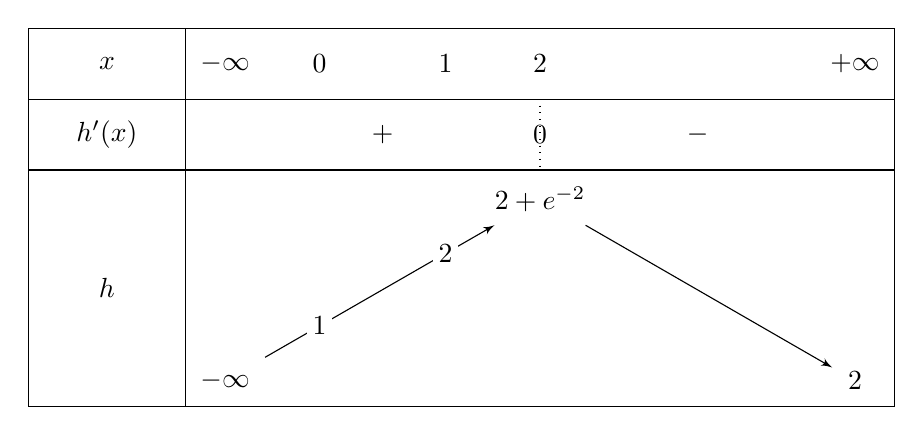
\begin{tikzpicture}
    % espcl=2 définit l'espace entre les colonnes
    \tkzTabInit[espcl=4]{$x$ / .9 , $h'(x)$ / .9, $h$ / 3}{$-\infty$, $2$, $+\infty$}
    
    % Ligne de la dérivée : s'annule en 2
    \tkzTabLine{, +, z, -, }
    
    % Ligne de la fonction : valeurs aux bornes et extremum
    \tkzTabVar{-/ $-\infty$, +/ $2+e^{-2}$, -/ $2$}
    
    % Placement des valeurs intermédiaires sur les flèches
    % \tkzTabVal{Début}{Fin}{Position(0 à 1)}{Valeur_X}{Valeur_Y}
    \tkzTabVal{1}{2}{0.3}{0}{$1$} % Place le 1 à environ 1/3 de la montée
    \tkzTabVal{1}{2}{0.7}{1}{$2$} % Place le 2 à environ 2/3 de la montée
\end{tikzpicture}
\end{center}

\begin{enumerate}
    \item On note $h'$ la dérivée de $h$. Calculer $h'(x)$ en fonction de $a$ et $b$.
    \item En utilisant les données numériques du tableau de variation de $h$ :
    \begin{enumerate}
        \item Déterminer les limites de $h$ en $-\infty$ et en $+\infty$.
        \item Démontrer que $a = 1$, $b = -1$ et $c = 2$. \\
        Ainsi donc dans la suite du problème $h(x) = (x - 1)e^{-x} + 2$.
    \end{enumerate}
    \item \begin{enumerate}
        \item Démontrer que l'équation $h(x) = 0$ admet une unique solution $\alpha$ dans $]-1; 0[$.
        \item En déduire le signe de $h(x)$.
    \end{enumerate}
\end{enumerate}

\vspace{0.5cm}

\noindent \underline{\textbf{Partie B}} \\
On note $(C_f)$ la courbe représentative de la fonction $f$ par $f(x) = 2x - 1 - xe^{-x}$. \\
(Unité : 2 cm)
\begin{enumerate}
    \item \begin{enumerate}
        \item Calculer la limite de $f$ en $+\infty$.
        \item Démontrer que la droite $(D)$ d'équation $y = 2x - 1$ est asymptote à $(C_f)$ en $+\infty$.
        \item Préciser les positions de $(C_f)$ par rapport à $(D)$.
    \end{enumerate}
    \item Calculer les limites en $-\infty$ de $f(x)$ et de $\dfrac{f(x)}{x}$. En donner une interprétation graphique.
    \item \begin{enumerate}
        \item Démontrer que $f'(x) = h(x)$.
        \item Donner le sens de variation de $f$ puis dresser le tableau de variation de $f$.
    \end{enumerate}
    \item \begin{enumerate}
        \item Démontrer que $f(\alpha) = 2\alpha + 1 + \dfrac{2\alpha}{\alpha - 1}$.
    \end{enumerate}
\end{enumerate}

\begin{comment}
\begin{center}
    \fbox{\textbf{\exo}}
\end{center}
\end{comment}
\end{document}